% Modelo Original a partir do template do trabalho do Aluno Tiago Augusto Gomes da Costa
% Prof Orientador Dr. Flávio Garcia Pereira
% 22/08/2019

\documentclass[12pt, openright, oneside, a4paper, english, french, spanish, brazil]{abntex2}
\usepackage[utf8]{inputenc}

\usepackage{lmodern}			% Usa a fonte Latin Modern			
\usepackage[T1]{fontenc}		% Selecao de codigos de fonte.
\usepackage[utf8]{inputenc}		% Codificacao do documento (conversão automática dos acentos)
\usepackage{lastpage}			% Usado pela Ficha catalográfica
\usepackage{indentfirst}		% Indenta o primeiro parágrafo de cada seção.
\usepackage{color,soul}			% Controle das cores
\usepackage{graphicx}			% Inclusão de gráficos
\usepackage{microtype} 			% para melhorias de justificação
\usepackage{amsmath}
\usepackage{afterpage}
\usepackage{subcaption}
\usepackage{textcomp}
\usepackage{hyperref}
%\usepackage{subfig}
\usepackage{gensymb}

\usepackage{float}

\usepackage{pdfpages}
\usepackage[section]{placeins}
\usepackage{amsfonts}

\usepackage{listings}           % Python Code
\usepackage{newfloat,tocloft}
\usepackage{caption}
\usepackage{enumitem}
\setlist{leftmargin=5.5mm}
\usepackage[explicit,nobottomtitles*]{titlesec}

\usepackage[brazilian,hyperpageref]{backref}	 % Páginas com as citações na bibl
\usepackage[alf, bibjustif]{abntex2cite}	% Citações padrão ABNT

% Formatação de Página
\usepackage[a4paper]{geometry}
\geometry{
 a4paper,
 left=30mm,
 top=30mm,
 bottom=20mm,
 right=20mm
}

% Formatação de Fonte
\renewcommand{\rmdefault}{phv} % Arial
\renewcommand{\sfdefault}{phv} % Arial

%% Formatação de Capítulo
\titleformat{\chapter}
  {\normalfont\normalsize\bfseries}{\thechapter \quad \MakeUppercase{#1}}{.5em}{\vspace{.5ex}}
  \titlespacing*{\chapter}      
    {0pt}{0pt}{12pt}
    
% Formatação de Seção
\titleformat{\section}
  {\normalfont\normalsize}{\thesection \quad #1}{.5em}{\vspace{.5ex}}

% Formatação de Subseção
\titleformat{\subsection}
  {\normalfont\normalsize}{\thesubsection \quad #1}{.5em}{\vspace{.5ex}}  

% Numeração
\makeevenfoot{plain}{}{}{\thepage}
\makeoddfoot{plain}{}{}{\thepage}

% Parágrafo
\setlength{\parskip}{1em}
\renewcommand{\baselinestretch}{1.5}

 % Início do TCC
\titulo{Ensaios de detec\c cão facial em dispositivos de borda, para monitoramento e controle de acesso em espa\c cos abertos e inteligentes}
\autor{Conrado Costa}
\data{2021} %deixar apenas o ano
\local{Serra -- ES}
\orientador{Prof. Rafael Emerick Z de Oliveira}
%\orientador[Orientadora:]{Prof\textsuperscript{a}. Dr\textsuperscript{a}. Nome da Orientadora}
%\coorientador{Prof. Dr. Nome do Coorientador}
%\coorientador[Coorientadora:]{Prof\textsuperscript{a}. Dr\textsuperscript{a}. Nome da Coorientadora}
\renewcommand{\backrefpagesname}{Citado na(s) página(s):~}

\begin{document}

{
    \center
    {\large\MakeUppercase{Instituto Federal do Espírito Santo}}
    \par
    \vspace{0.5cm}
    {\large\MakeUppercase{Engenharia de Controle e Automação}}
    \par
    %{\large\MakeUppercase\imprimircurso}
    %\par
    \vfill
    {\large\MakeUppercase\imprimirautor}\par
    \vfill
    {\bfseries\large\MakeUppercase\imprimirtitulo}\par
    \vfill
         
    \vfill
    {\large\MakeUppercase\imprimirlocal}\par
    {\large\imprimirdata}\par
}


\newpage

{
\center          
{\large\MakeUppercase{\imprimirautor}}\par
\vfill
{\bfseries\large\MakeUppercase\imprimirtitulo}\par
\vspace{10 mm}
\hspace{.35\textwidth}
\begin{minipage}{.6\textwidth}
    \SingleSpacing
    Trabalho de conclusão de curso, apresentada como parte das atividades para obtenção do título de bacharel em Engenharia de Controle e Automação, do curso de Engenharia de Controle e Automação do Instituto Federal do Espírito Santo. 
    \par
    \par
    \vspace{0.5cm}
    \imprimirorientadorRotulo
    {\large  } \imprimirorientador\par
    \imprimircoorientadorRotulo
    {\large  } \imprimircoorientador\par
\end{minipage}
\vfill 
\vfill
{\large\MakeUppercase\imprimirlocal}\par
{\large\imprimirdata}\par
}
Aqui entra a Ficha catalográfica.

Será gerada pela biblioteca!

\setcounter{page}{1}
\pagenumbering{arabic}                % arabic numbers <-----------------(style 1,2,...)
\pagestyle{empty}

{
    \center          
    {\large\MakeUppercase{\imprimirautor}}\par
    \vfill
    {\bfseries\large\MakeUppercase\imprimirtitulo}\par
    \vspace{10 mm}
    \hspace{.35\textwidth}
    \begin{minipage}{.6\textwidth}
        \SingleSpacing
        Texto submetido ao Curso de Graduação em Engenharia de Controle e Automação do Instituto Federal do Espírito Santo como requisito parcial para obtenção do título de Bacharel em Engenharia de Controle e Automação. 
    \end{minipage}
    
    \vspace{1.5cm}
    
    Aprovada em XX de XXXXX de XXXX.
    
    \vspace{1.0cm}
    
    \MakeUppercase{Comissão Examinadora}
    
    \vspace{1.0cm}
    
    \rule{12cm}{1pt} \\
    Prof. Rafael Emerick Z de Oliveira \\
    Instituto Federal do Espírito Santo - \textit{campus} Serra
    
    \vspace{1.0cm}
    \rule{12cm}{1pt} \\
    Prof. XXXXX \\
    Instituto Federal do Espírito Santo - \textit{campus} Serra
    
    \vspace{1.0cm}
    \rule{12cm}{1pt} \\
    Prof. XXXXX \\
    Instituto Federal do Espírito Santo - \textit{campus} Serra
    
%    \vspace{1.0cm}
%    \rule{12cm}{1pt} \\
%    Prof. Dr. Fulano de Tal \\
%    UCL
    
    \vfill 
    \vfill
    {\large\MakeUppercase\imprimirlocal}\par
    {\large\imprimirdata}\par
}
{
\begin{center}
    \MakeUppercase{Declaração do Autor}
\end{center}

}

\vspace{1cm}

Declaro, para fins de pesquisa acadêmica, didática e técnico-científica, que a presente Dissertação de Mestrado pode ser parcial ou totalmente utilizada desde que se faça referência à fonte e aos autores.

\vfill

\begin{center}
    \rule{12cm}{1pt} \\
    \imprimirautor    
    
    \vfill
    
    Serra, XX de XXXXX de XXXX.
\end{center}






%\begin{minipage}{1cm}

\end{minipage}

\vfill

\begin{flushright}
Para meu pai e minha mãe.
\end{flushright}
%\chapter*{Agradecimentos}

Escreva seus agradecimentos aqui.
%\begin{minipage}{1cm}

\end{minipage}

\vfill

\begin{center}
\begin{minipage}{11cm}
``Texto da epígrafe.''
\end{minipage}
\end{center}

\vspace{1.5cm}

\begin{flushright}
Autor da frase.
\end{flushright}



\begin{resumo}

<a preencher>
 
\vspace{0.5cm}
 
 \textbf{Palavras-chave:} Processamento Digital de Imagens; Inteligência Artificial; Rede Neural; Máquina de Vetor de Suporte; 
\end{resumo}
\captionsenglish

\begin{resumo}
 
<a preencher> 
 
 \vspace{0.5cm}
 
 \textbf{Keywords:} Digital Image Processing; Artificial Intelligence; Neural Network; Support Vector Machine. 
\end{resumo}
\captionsbrazil

%\listoftables
%\newpage

\listoffigures
\newpage

\tableofcontents

\graphicspath{{Figuras/}}

\pagestyle{plain}

%\setcounter{page}{13} %Ajustar esse número de acordo com a numeração da sua página

\chapter{Introdução}
\label{chap:intro}
\thispagestyle{plain}

O problema de segurança pública sempre foi um problema sério no Brasil. Constantes crimes de furtos e roubos geram grande danos, principalmente financeiros, tanto para o indivíduo, no caso das vítimas, quanto para a sociedade \cite{Cerqueira2007, G12013}. Um dos reflexos gerados por essa insegurança está no fato de que vários locais públicos devem ter seu acesso controlado e vigiado para garantir a segurança patrimonial.

As \textit{smart cities} (cidades inteligentes) estão emergindo como uma prioridade para pesquisa e desenvolvimento em todo o mundo. Elas abrem oportunidades significativas em várias áreas, como crescimento econômico, saúde, bem-estar, eficiência energética e transporte, para promover o desenvolvimento sustentável das cidades \cite{Song2017}. O conceito e oportunidades das \textit{smart cities} são escaláveis para outros conceitos ‘smart’ como o \textit{smart room}, \textit{smart home}, \textit{smart building}, etc \cite{Pacheco2018}. A proliferação de tecnologias de informação e comunicação possibilita o desenvolvimento de diversos serviços inteligentes. E um dos serviços comunitários mais essenciais é justamente a vigilância inteligente \cite{Chen2016, Nikouei2018}.

Nos últimos anos, aplicações de reconhecimento facial a partir de imagens geradas por câmeras de videomonitoramento têm ganhado relevância, sendo largamente utilizadas para a verificação ou identificação de indivíduos em locais públicos. No âmbito da segurança, o reconhecimento facial em vídeo permite agilidade nas situações em que muitos indivíduos devem ser identificados rapidamente \cite{Quirita2014}.

Apesar de estarmos longe de conseguir com que a IA (inteligência artificial) se aproxime da performance humana, em algumas áreas, como reconhecimento de imagem, carros autônomos e jogos eletrônicos, ela se mostra equivalente, ou até mesmo superior \cite{Aggarwal2018}. Em tarefas de visão computacional é possível rastrear o movimento de uma pessoa em um plano de fundo complexo. E com moderado sucesso, é possível tentar localizar e nomear todas as pessoas em uma fotografia, através da detecção e reconhecimento de faces, roupas e cabelos \cite{Szeliski2011}.

O \textit{deep learning} (aprendizagem profunda), ramo do \textit{machine learning} (aprendizagem de máquina), tornou-se imensamente popular no reconhecimento de imagens, bem como em outras tarefas de reconhecimento e correspondência de padrões \cite{Verhelst2017}.

As redes neurais artificiais simulam o sistema nervoso humano com base em aprendizado de máquina, tratando as unidades computacionais em um modelo de aprendizado de maneira semelhante aos neurônios humanos. Não é uma tarefa fácil pois o poder computacional do computador mais rápido atualmente equivale a uma pequena fração do poder computacional de um cérebro humano \cite{Aggarwal2018}. 

As \textit{deep neural networks} (redes neurais profundas) envolvem uma complexidade computacional significativa, fazendo com que, até recentemente, seu processamento fosse viável apenas em plataformas de potentes servidores disponíveis na ‘nuvem’ \cite{Verhelst2017}. Quando é necessário armazenamento e computação de dados em larga escala, a computação em nuvem tem sido a solução. Porém, com o grande crescimento de dispositivos móveis e inteligentes, juntamente com as tecnologia de IoT (Internet das Coisas), o foco mudou para se obter respostas em tempo real. \cite{Dolui2017}.

Nos últimos anos, vê-se uma tendência de se incorporar o processamento de aprendizado profundo em dispositivos de borda, como celulares, dispositivos móveis e nos nós da IoT. Isso torna possível a análise de dados localmente, em tempo real, além de mitigar problemas de privacidade dos dados \cite{Verhelst2017}. Outro benefício da computação na borda (\textit{Edge Computing}) é o descongestionamento da rede de dados, pois permite que o processamento seja feito próximo das fontes dos dados \cite{Merenda2020}. Assim, evita-se a comunicação desnecessária, que sobrecarrega não só a rede principal como também o datacenter na nuvem \cite{Aazam2014}.

\section{Objetivo Geral}

Com este trabalho objetiva-se testar o desempenho de dispositivos de borda no processo de detecção de faces, avaliando sua capacidade de detecção e tempo de resposta para diferentes cenários, com possíveis aplicações de monitoramento inteligente e controle de acesso. Com os resultados obtidos, espera-se determinar, para cada cenário definido, se o dispositivo é capaz de processar de forma satisfatória a etapa de detecção de faces, e as vantagens de se realizar esse processo na borda, em uma arquitetura de processamento distribuído.

\subsection{Objetivos Específico}
Em um sentido mais estrito, pretende-se
\begin{itemize}
    \item Definir diferentes cenários (com aplicabilidade para monitoramento inteligente e controle de acesso) e os requisitos a serem cumpridos, como tempos de respostas e capacidade de reconhecimento. Serão utilizadas imagens estáticas que representem cada cenário para os testes.
    \item Desenvolver uma ferramenta cliente-servidor para auxiliar na parametrizacão do algoritmo de detecção, buscando melhor otimização para cada cena e dispositivo, e na obtenção das métricas de desempenho.
    \item Analisar os resultados obtidos e determinar para quais cenários os dispositivos podem executar a detecção de face de forma satisfatória e quais os ganhos em se executar tal processamento na borda, principalmente no que se refere à utilização de banda na rede de um sistema com arquitetura de processamento distribuído, sua escalabilidade e tempos de resposta.
\end{itemize}

\section{Estrutura do Texto}
<a preencher>
%Para a exposição do trabalho realizado, este texto foi dividido em cinco capítulos, sendo o Capítulo 1, Introdução, responsável pela apresentação do texto bem como por situar o leitor no contexto ao qual este trabalho se insere. No Capítulo 2, Revisão Teórica, são apresentados alguns conceitos que serão necessário ao bom entendimento das técnicas e soluções propostas. O capítulo 3, Desenvolvimento, explica qual a abordagem utilizada diante do problema, exibindo as diferentes etapas envolvidas na solução do problema, enquanto que o Capítulo 4, Experimentos Realizados, mostra a implementação do sistema proposto. Por fim os resultados obtidos são avaliados e discutidos no Capítulo 5, de nome Conclusão.
\chapter{Revisão Teórica}
\label{cap:rev.teorica}
\thispagestyle{plain}
\graphicspath{{./Cap2_Revisao_Teorica/Figures/}}

\section{O problema da segurança em espaços públicos e privados}
O problema de segurança pública no Brasil é algo que está sempre em evidência. O Programa das Nações Unidas para o Desenvolvimento (Pnud), em seu relatório divulgado em 12/11/2013, constata que o Brasil apresentou a maior taxa de roubo da América Latina, segundo dados de 2011 repassados pelos países. Os dados apontam que para cada 100 mil habitantes no Brasil, há 572,7 ocorrências de roubo. E sabe-se que, na realidade, esse número tende a ser maior, tendo em vista que nem todos os roubos são reportados às autoridades \cite{G12013}.

Estima-se um total de 15 milhões de ocorrências de roubos e furtos no Brasil no ano de 2003, incluído os casos que não foram notificados. E como parte da consequência, estima-se uma perda material de R\$ 8,4 bilhões \cite{Cerqueira2007}. Se corrigido para o ano de 2020 com base no IPCA (Índice de Preços ao Consumidor Amplo), esse valor seria de aproximadamente R\$ 20,2 bilhões. Esse cálculo foi feito com base em uma calculadora online disponível no site do Banco Central do Brasil (BCB). Esse é um problema que gera não só perdas para as vítimas dos roubos e furtos, mas também indiretamente para outros indivíduos da sociedade, uma vez que, essa transferência de valor pode ser considerada como recurso de oportunidade a serem aplicados no setor de crimes. Este, por sua vez, demanda recurso público para o seu combate, tornando o problema um causador não só de dano ao indivíduo, como também de custo social \cite{Anderson1999, Cerqueira2007}.

Os fatores que motivam ou favorecem esse tipo de crime são vários. A teoria das janelas quebradas, testada em um experimento por Philip Zimbardo, psicólogo de Stanford, propõe-se a explicar um deles. O experimento consistiu em deixar dois carros similares abandonados nas ruas de dois bairros diferentes de Nova Iorque, um nobre e outro na periferia. O que se observou foi quem o carro deixado na periferia foi atacado por vândalos nos primeiros 10 minutos, enquanto o segundo carro, deixado no bairro nobre, ficou intocado por mais de uma semana. Então Zimbardo com uma marreta danificou parte do carro e o que se observou em seguida foi que várias pessoas que estavam transitando se juntaram ao carro, que, em poucas horas, estava completamente destruído.  O que o experimento transmite é que a desordem e o crime estão de certa forma ligados. A desordem passa uma impressão de descuido, de forma que um indivíduo mal intencionado se sentirá muito mais à vontade em cometer algum delito, por ter a sensação de que ninguém irá notar, ou se importar. E por isso, há também uma sensação de impunidade. Uma propriedade mal cuidada se torna ideal para os que saem na intenção de vandalizar ou saquear, e até mesmo para aqueles quem nem pensariam em tais atitudes, mas as cometem ao enxergar o delito como uma oportunidade \cite{Wilson1982}.

Sistemas de câmeras de vigilância têm sido cada vez mais implantados em muitos lugares, como prédios, ruas, instalações industriais e comerciais, escolas, shoppings, aeroportos e residências, provendo, segurança pública, monitoramento de ambientes internos, monitoramento de tráfego e proteção de infraestrutura \cite{Puvvadi2015}.

Em uma das formas de monitoramento, as imagens da câmera são monitoradas em tempo real por seguranças. Como outra forma, é possível registrar a saída de cada câmera no um gravador (VCR), para futura análise. Porém, na primeira forma de monitoramento, uma ocorrência ou incidente de segurança pode acabar não sendo verificado, devido, por exemplo, a uma falha humana. E no segundo caso, o momento da verificação do ocorrido pode não acontecer em um tempo satisfatório \cite{Olson2006, RamosLima2019}. Mas hoje, com o avanço da tecnologia, temos opções mais inteligentes de monitoramento, como é tratado no item 1.2.

\section{\textit{Smart cities} e videomonitoramento inteligente}

“Smart City” é um poderoso paradigma que aplica as mais avançadas tecnologias de comunicação aos ambientes urbanos, com o objetivo de melhorar a qualidade de vida nas cidades e fornecer um amplo conjunto de serviços de valor tanto para os cidadãos quanto à administração \cite{Cenedese2014}. O recente conceito de Smart Cities, impulsionado pelo rápido crescimento da IoT (Internet das Coisas), atraiu a atenção de planejadores urbanos e pesquisadores para aumentar a segurança e o bem-estar dos residentes. A proliferação de tecnologias de informação e comunicação conecta sistemas ciber-físicos e entidades sociais, bem como possibilita muitos sistemas inteligentes. Um dos serviços comunitários inteligentes mais essenciais é a vigilância inteligente \cite{Chen2016, Nikouei2018}.

Nos últimos tempos, os sistemas de câmeras de vigilância evoluíram de simples aquisição de vídeo e sistemas de exibição para sistemas semiautônomos inteligentes, capazes de realizar procedimentos complexos. Hoje em dia, um sistema de vigilância por vídeo pode integrar alguns dos algoritmos de análise de imagem e vídeo mais sofisticados como de classificação (por exemplo, redes neurais), reconhecimento de padrões, tomada de decisão, aprimoramento de imagem e vários outros \cite{Tsakanikas2018}. Isso permite uma grande possibilidade de aplicações como controle de acesso em áreas de interesse, reconhecimento de faces humanas, detecção de padrões e objetos, reconhecimento de comportamento, estatísticas de fluxo de multidões, análise de congestionamento, etc \cite{Hu2004}.

Um sistema de vigilância moderno compreende não só dispositivos de aquisição de imagem e vídeo para exibição, mas também dispositivos para processamento de dados e unidades de armazenamento, componentes cruciais para a execução da tarefa \cite{Tsakanikas2018}. Além disso, têm estado cada vez mais disponíveis dispositivos de vigilância com conectividade de rede que suportam o protocolo IP. Isso abre uma ainda maior gama de possibilidades já que os dados podem ser enviados praticamente para qualquer de equipamento onde quer que este esteja localizado. Porém, isso traz junto a preocupação com a privacidade, pois os dados de imagem trafegados em rede estão sujeitos a interceptações. Uma abordagem utilizada é a criptografia dos dados em tráfego, porém isso traz uma carga maior de processamento que pode acabar prejudicando a performance do monitoramento em tempo real \cite{Puvvadi2015}. 

Muitas das aplicações de videomonitoramento inteligente requerem recursos computacionais e de armazenamento significativos, para ser capaz de lidar com a grande quantidade de dados gerada pelos sensores de vídeo. De acordo com o estudo recente, os dados de vídeo dominam o tráfego em tempo real e criam uma carga de trabalho pesada nas redes de comunicação. Por exemplo, vídeo online responde por 74\% de todo o tráfego online em 2017 e 78\% do tráfego móvel será de dados de vídeo em 2021. O volume de dados são cada vez maiores, à medida que se têm maiores taxas de quadro e maiores resoluções \cite{Porter2010}.

O paradigma da computação em nuvem, ou Cloud Computing, oferece excelente flexibilidade para lidar com essa grande quantidade de transferência de dados, além de também de ser escalável, correspondendo ao número crescente de câmeras de vigilância \cite{Nikouei2018}. Para tarefas de vigilância urbana que requerem a combinação de dados complexos, a computação em nuvem têm sido amplamente aceita como a solução \cite{Chen2016}. No entanto, existem obstáculos significativos para a arquitetura de vigilância inteligente baseada em nuvem remota \cite{Nikouei2018}. Os delay adicional devido à comunicação em rede pode não ser tolerável em aplicações que sejam sensíveis a latências mais altas, como as aplicações de tempo real \cite{Chen2016}. Uma grande distância entre o sensor de vídeo e os servidores da nuvem, além dos possíveis congestionamentos na rede, torna ainda mais inviável essa abordagem.

\section{Redes Neurais e Deep Learning}
Deep Learning, ou aprendizado profundo, é um campo do aprendizado de máquina baseado nas em redes neurais artificiais \cite{Brownlee2019}.

“Redes neurais artificiais são técnicas populares de aprendizado de máquina que simulam o mecanismo de aprendizado em organismos biológicos. O sistema nervoso humano contém células, conhecidas como neurônios. Os neurônios são conectados uns aos outros com o uso de axônios e dendritos, e as regiões de conexão entre os axônios e dendritos são chamadas de sinapses” \cite{Aggarwal2018}.

Na programação convencional, o programador, através de várias linhas precisas de código, determina quais tarefas que o computador deve executar, à risca. Grandes problemas são quebrados em problemas menores nos quais os computadores conseguem performar. Já no paradigma de redes neurais, o programador não precisa dizer exatamente o que a máquina deve fazer. Ao invés disso, a partir de algoritmos de aprendizado e dados observacionais, a máquina consegue aprender por si só como resolver determinado problema \cite{Neapolitan2018}.

Existem várias diferentes arquiteturas de redes neurais que são comumente usadas em diferentes aplicações, como as \textit{Restricted Boltzmann Machines} (RBM), as \textit{Recurrent Neural Networks} (RNN) e as \textit{Convolutional Neural Networks} (CNN). As mais utilizadas atualmente são as CNN e as RNN. As RNN, ou redes neurais recorrentes, são projetadas para trabalhar com dados sequenciais, como frases de texto, séries temporais e outras sequências discretas, como sequências biológicas. As CNN, ou redes neurais convolucionais, são redes inspiradas biologicamente e são usadas em visão computacional para classificação de imagens e detecção de objetos. \cite{Aggarwal2018}.

As redes neurais convolucionais têm se mostrado a mais bem-sucedidas de todos os tipos de redes neurais. São amplamente usadas para o reconhecimento de imagem, detecção de objetos, rastreamento e até mesmo processamento de texto. O desempenho dessas redes chegou a superar o desempenho dos humanos no problema de classificação de imagens \cite{He2016}.

Existem hoje disponíveis gratuitamente vários frameworks e estruturas de aprendizado de máquina incluindo redes neurais, tornando o trabalho de treinar uma rede neural mais simples. Entre as mais conhecidas estão Keras, PyTorch, TensorFlow, Scikit-learn. O treinamento de redes neurais exige muito poder de processamento. Os cálculos de deep learning tendem a ser mais rápidos quando feitos por GPUs (\textit{Graphical Processing Units}) \cite{Heller2019}.


\section{Processamento de imagens, detecção e reconhecimento de faces}
Pesquisadores têm desenvolvido na área de visão computacional técnicas matemáticas para recuperar a forma tridimensional e a aparência de objetos em imagens. Hoje, há técnicas confiáveis para calcular com precisão um modelo 3D parcial de um ambiente a partir de milhares de fotografias sobrepostas. A visão computacional é usada hoje em uma ampla variedade de aplicativos do mundo real, que incluem reconhecimento óptico de caractere (OCR), segurança automotiva, videomonitoramento, reconhecimento de digitais, detecção e reconhecimento de faces, entre outros \cite{Szeliski2011}.

A detecção de faces é um problema já bem resolvido na área de visão computacional. Isso deve-se ao fato de que a detecção de faces é um dos processos mais utilizados em sistemas de videomonitoramentos e é exigido em vários tipos de aplicações como reconhecimento de faces, rastreamento, análise comportamental, etc \cite{Zafeiriou2015}.

“O objetivo da detecção de face é, em primeiro lugar, determinar se algum rosto está representado em uma cena e, em segundo lugar, calcular e retornar as coordenadas dos rostos detectados. Esta tarefa envolve muitas condições não triviais, como variações de escala, localização, orientação e pose, bem como condições de iluminação, expressões faciais e oclusões” \cite{Tsakanikas2018}.

Entre várias técnicas detecção de face, o trabalho inovador de Viola e Jones (Viola and Jones, 2001) baseado em melhorar o processo de detecção de faces, foi o primeiro algoritmo que tornou a detecção de rosto praticamente viável em aplicações do mundo real. Até hoje é amplamente aplicada em câmeras digitais e softwares de organização de fotos \cite{Zafeiriou2015}. A abordagem proposta por Viola e Jones para detecção de objetos minimiza o tempo de processamento ao mesmo tempo em que consegue grande acurácia na detecção. E quando aplicado na detecção de faces, se mostrou 15 vezes mais rápido que qualquer abordagem precedente \cite{Viola2001}. A biblioteca OpenCV, multiplataforma e de uso totalmente livre (OpenCV),  disponibiliza uma função de detecção de objeto baseada no método proposto por Viola e Jones.

O reconhecimento de faces constitui o problema de identificar a face de uma pessoa mediante a comparação com uma base de dados de inúmeras outras faces previamente identificadas, a partir da qual obtém-se o grau de similaridade entre cada comparação \cite{Quirita2014}. O problema de reconhecimento de face requer que um rosto já tenha sido detectado em uma imagem, portanto, a detecção de face se torna um pré-requisito para o processo de reconhecimento. Nos últimos tempos, os algoritmos de reconhecimento de faces evoluíram de tal forma que hoje podem ser usados em aplicativos do mundo real e em ambientes não controlados. \cite{Zafeiriou2015}.

Uma das primeiras abordagens para reconhecimento de face baseia-se em localizar as características distintas da imagem, como olhos, nariz, boca, e medir a distância entre as posições de cada uma \cite{Fischler1973, Kanade1977}. Abordagens mais recentes baseiam-se na comparação de imagens em escala de cinza projetadas em subespaços dimensionais inferiores chamados de eigenfaces \cite{Szeliski2011}.

Um sistema de reconhecimento de faces, baseado em características, geralmente consiste de quatro partes: detecção, alinhamento, extração de características e combinação/verificação, conforme é esquematizado na figura 2.1 \cite{StanZ.Li2011}.

\begin{figure}[h]
    \centering
    \caption[Fluxo de processo de reconhecimento de face.]{Fluxo de processo de reconhecimento de face }
    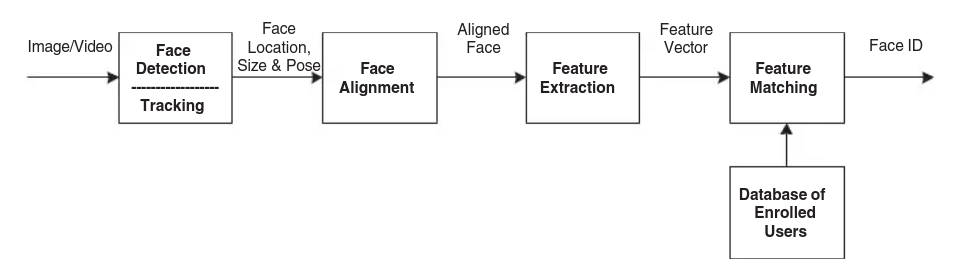
\includegraphics[width=0.8\textwidth]{Cap2_Revisao_Teorica/Figures/fluxo_rec.png}
    \caption*{Fonte: \cite{StanZ.Li2011}}
    \label{fig:fluxoReconhecimento}
\end{figure}

Na etapa de detecção “Face Detection”, temos um vídeo ou uma imagem como entrada. Essa etapa tem como função localizar e extrair uma ou mais faces que estejam presentes na imagem. No caso em que a entrada é um vídeo, se necessário, essa etapa também é responsável pelo rastreamento, “Tracking”, das faces, quadro a quadro. A faces extraídas passam então pela etapa de alinhamento, “Face Alignment”, que é responsável por normalizar a imagem em rotação e em escala, de forma que na imagem resultante a face esteja alinhada ao eixo horizontal do plano. \cite{StanZ.Li2011, Quirita2014}.

Depois de já alinhada, a face passa pela etapa de extração de características, “Feature Extraction”. Essa etapa tem a função de identificar e extrair da face pontos faciais distintos, como olhos, nariz, boca e outras marcas de referência que sejam suficientes para caracterizar a face, de forma que a mesma possa ser distinguida dentre as faces obtidas de outras pessoas. \cite{StanZ.Li2011}. Em seguida são computadas as relações geométricas entre esses pontos faciais, reduzindo-se assim a imagem facial de entrada em um vetor de características geométricas \cite{Jafri2009}. A figura 2.2 destaca alguns pontos faciais característicos e as relações geométricas entre eles.

Os primeiros trabalhos realizados em reconhecimento de faces baseavam-se principalmente nessa técnica. Em uma das primeiras tentativas empregou-se um método simples de processamento de imagem para extrair um vetor de 16 parâmetros faciais, que eram relações de distâncias, áreas e ângulos, de forma a compensar o tamanho variável das imagens. Então usou-se uma medida de distância euclidiana simples para correspondência, chegando a um desempenho máximo de 75\% em um banco de dados de 20 pessoas diferentes, usando 2 imagens por pessoa. \cite{Kanade1977}

\begin{figure}[h]
    \centering
    \caption[Características geométricas (destaque em branco), usada em experimentos de reconhecimento de faces.]{Características geométricas (destaque em branco), usada em experimentos de reconhecimento de faces}
    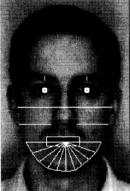
\includegraphics[width=0.2\textwidth]{Cap2_Revisao_Teorica/Figures/face_vetores.png}
    \caption*{Fonte: \cite{StanZ.Li2011}}
    \label{fig:faceVetores}
\end{figure}

Tendo as características geométricas da face calculadas e codificadas em um vetor, a próxima etapa para o reconhecimento da face é fazer a correspondência, ou “Feature Matching” (quarta e última etapa do processo de reconhecimento proposto na figura 1.2). Essa etapa consiste em comparar o vetor obtido da face que se deseja reconhecer com um banco de dados de vetores de outras faces que já são conhecidas e tiveram suas caraterísticas extraídas pelo mesmo processo descrito até aqui. O reconhecimento é feito com base no grau de similaridades entre a face sendo verificada e as faces conhecidas \cite{Quirita2014}.   

A principal vantagem oferecida pelas técnicas de reconhecimento baseadas em características é que, uma vez que a extração dos pontos característicos é anterior à análise feita para comparar a face com a de um indivíduo conhecido, esses métodos são relativamente robustos para variações de posição na imagem de entrada \cite{Jebara1996}. A princípio, esquemas baseados em características podem ser invariáveis ao tamanho, orientação ou iluminação \cite{Cox1996}. Outras vantagens de se utilizar técnicas baseadas em características faciais incluem a compactação de representação das imagens de face e a alta velocidade na tarefa de verificação de correspondência (identificação) \cite{Brunelli1992}.

A principal desvantagem dessa técnica é a dificuldade de detecção automática de características e o fato de que o desenvolvedor da aplicação deve tomar decisões arbitrárias sobre quais características são importantes para o processo de reconhecimento \cite{Cendrillon2000}.

A biblioteca Dlib C++ disponibiliza algumas ferramentas para reconhecimento facial. Em seu site, está disponível gratuitamente um modelo pré-treinado para extração de características faciais, que alcançou uma marca de precisão de 99,38\% no benchmark de reconhecimento facial da \textit{Labeled Faces in the Wild} (LFW), que é comparável a outros métodos de última geração para reconhecimento facial em fevereiro de 2017. \cite{Dlib}. A LFW é uma referência pública para verificação de desempenho de reconhecimento facial \cite{Lfw}.

Esse modelo mapeia a imagem de uma face humana em um vetor de 128 dimensões espaciais. Quando vetores de duas imagens diferentes são muito próximos, significa que a face tende a pertencer à mesma pessoa. Assim, o reconhecimento facial pode ser obtido mapeando-se várias faces em vetores de 128 dimensões e compará-las entre si calculando a distância Euclidiana \cite{Dlib}.

Esse modelo foi treinado a partir de um banco de cerca de 3 milhões de imagens. A precisão alcançada de 99,38\% significa que, ao ser apresentada um par de imagens faciais, a ferramenta identificará corretamente se o par pertence à mesma pessoa ou é de pessoas diferentes  em 99,38\% das vezes \cite{Dlib}, o que o torna uma boa ferramenta para reconhecimento de faces de uma forma geral.

O grande avanço nas técnicas e ferramentas de aprendizado de máquina abriu um grande leque de possibilidades de aplicações de inteligência artificial nos últimos anos. Devido a isso, os recentes modelos de detecção e reconhecimento, não só de faces, mas de objetos em geral, estão cada vez mais precisos e rápidos. Isso, aliado ao expressivo avanço da Internet das Coisas (IoT), trazendo à tona o conceito de Edge Computing, torna cada vez mais viável as implementações de videomonitoramento automático.


\section{A Internet das Coisas, Edge e Fog Computing}

A Internet das Coisas, ou Internet of Things (IoT), é um paradigma de comunicação recente que prevê em um futuro próximo que os objetos da vida cotidiana serão equipados com microcontroladores, transceptores para comunicação digital e pilhas de protocolo adequadas que os tornarão capazes de se comunicarem entre si e com os usuários finais, tornando-se parte integrante da Internet \cite{Atzori2010}.

O conceito de IoT, portanto, visa tornar a Internet ainda mais imersiva e abrangente. Além disso, ao permitir fácil acesso e interação com uma ampla variedade de dispositivos, como, por exemplo, eletrodomésticos, câmeras de vigilância, sensores de monitoramento, atuadores, monitores, veículos e assim por diante, a IoT promoverá o desenvolvimento de uma série de aplicações que fazem uso da quantidade e enorme variedade de dados gerados por tais objetos para fornecer novos serviços aos cidadãos, indústrias e administrações públicas. Esse paradigma encontra aplicação em muitos domínios diferentes, como automação residencial, automação industrial, assistência médica, saúde móvel, assistência a idosos, gerenciamento de energia inteligente e redes inteligentes, automotivo, gerenciamento de tráfego e muitos outros \cite{Bellavista2013}.

Com o advento da Internet das coisas nós estamos em uma era onde haverá uma grande quantidade de dados gerados por coisas que estão imersas em nosso dia a dia. Conforme estimado pelo Cisco Global Cloud Index, em 2019, os dados produzidos por pessoas, máquinas e “coisas” chegaria a 500 zetabytes \cite{Cisco2016}. Para processar esses todos esses dados, é necessário muito poder computacional.

Hoje em dia, a computação em nuvem é uma plataforma econômica e prevalecente, oferecendo enorme poder de processamento e capacidade de armazenamento para treinamento de modelos de machine learning, reconhecimento facial, reconhecimento de fala, visão computacional, processamento automatizado de linguagem, classificação de texto e diversas aplicações de IoT e smart cities. No entanto, também tem algumas desvantagens importantes, como latência de resposta da rede e a segurança do sistema no que diz respeito a questões de privacidade, já que para chegar na nuvem os dados, possivelmente sensíveis, precisam trafegar por um longo caminho na rede mundial \cite{Pacheco2018}.

A maioria das ações de controle de IoT deve ser realizada em tempo real, portanto, o tempo de espera de processamento em nuvem, principalmente devido à latência da rede, não funciona bem para problemas de IoT \cite{Singh2017}. Na tentativa de contornar algumas dessas limitações, aparecem alguns paradigmas recentes e complementares. São o Fog e o Edge Computing, que promete a capacidade de realizar tarefas de uma forma mais distribuída e responsiva, uma vez que os nós de IoT estão mais próximos das fontes de dados dos sensores. Além disso, também reduz o tráfego de rede e evita a exposição de dados privados do usuário \cite{Pacheco2018}.

A figura 2.3 demonstra muito bem a ideia de uma arquitetura de processamento distribuído, indicando as características que cada parte da rede dá à aplicação ao ser responsável por parte do processamento.
\begin{figure}[H]
    \centering
    \caption[Arquitetura de computação distribuída]{Arquitetura de computação distribuída}
    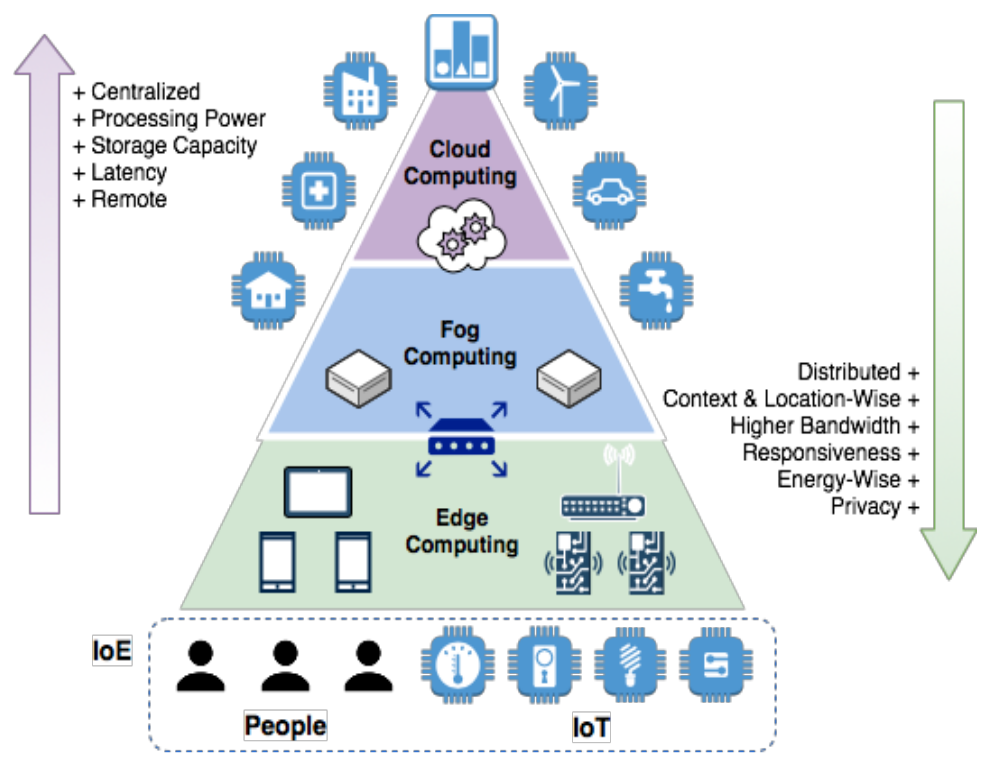
\includegraphics[width=0.9\textwidth]{Cap2_Revisao_Teorica/Figures/arquitetura_distribuida.png}
    \caption*{Fonte: \cite{Pacheco2018}}
    \label{fig:arquitetura}
\end{figure}


\chapter{Desenvolvimento}
\thispagestyle{plain}
\label{cap:desenvolvimento}
\graphicspath{{./Cap3_Desenvolvimento/Figures/}}

\section{O algoritmo de detecção de objetos}

O algoritmo de detecção de objetos utilizado nesse estudo foi o \textit{Haar cascade object detection}, proposto por Viola e Jones em sua pesquisa \textit{Rapid Object Detection using a Boosted Cascade of Simple Features} \cite{Viola2001}.

<pending>explicar um pouco sobre o algoritmo (baseado na detecção com base em características, é treinado com imagens positivas e negativas, É rapido pois a classificaçao em camadas descarta rapidamente uma area em que não há face, etc).</pending>

Não é o algoritmo com melhor acurácia atualmente, se comparado com técnicas mais modernas que aplicam \textit{deep learning}, porém é um algoritmo extremamente rápido e preciso, portanto ainda é muito útil para detecção de objetos em dispositivos com recursos limitados, como é o caso de dispositivos de borda, em geral.

Uma desvantagem nesse algoritmo é a tendência à detecção de falsos positivos e à necessidade de definição de alguns parâmetros, descritos resumidamente a seguir.

<pending>- parametros importantes (explicar cada)
--scaleFactor	Parameter specifying how much the image size is reduced at each image scale.
--minNeighbors	Parameter specifying how many neighbors each candidate rectangle should have to retain it.
--minSize	Minimum possible object size. Objects smaller than that are ignored.
--maxSize	Maximum possible object size. Objects larger than that are ignored. If maxSize == minSize model is evaluated on single scale.</pending>

O ajuste de parâmetros não é muito simples e depende do cenário da imagem, dos possíveis tamanhos de faces que se dejesa detectar, etc. A escolha dos parâmetros influencia diretamente no resultado da detecção, na capacidade de detecção de determinados tamanhos de faces, na propensão em detectar falsos-positivos e no tempo de execução.

Devido a isso, viu-se necessário o desenvolvimento de uma ferramenta para se testar de uma só vez um range variável de valores de determinados parâmetros e verificar facilmente a qualidade e tempo de detecção para cada conjunto de valores testados. 


\section{Ferramenta de parametrização, otimização e obtenção de resultados}

O \textit{design} da ferramenta foi pensado de forma a facilitar a análise do resultado de diversas combinações de parâmetros ao mesmo tempo, de diferentes imagens e em dispositivos diferentes, através de uma interface web.

Contitui de duas partes: a parte cliente, uma interface web que pode ser executada em qualquer dispositivo através de um navegador, e a parte servidor, que deve rodar nos dispositivos que serão testados.

No cliente é feita a seleção da imagem a ser utilizada no teste, é definido o endereço do dispositivo a ser testado, rodando o servidor, e são definidos os parâmetros de testes. O cliente envia os dados para o servidor que executa o algoritmo de detecção conforme os parâmetros passados e retorna para o cliente o resultado de cada combinação de valores dos parâmetros solicitados. O resultado é composto por uma matriz contendo o tempo médio de execução, a quantidade de faces detectadas e a posição de cada face detectada para cada par de valores dos parâmetros na matriz. As faces detectadas são vizualizadas na imagem ao se selecionar um dos resultados, permitindo, assim, a verificação da qualidade da de detecção e a presença de falsos-positivos.

Na figura a seguir temos um exemplo da interface com imagem e parâmetros selecionados, ainda sem exibição do resultado da análise.

\begin{figure}[h]
    \centering
    \caption[Interface e seus parâmetros.]{Interface e seus parâmetros.}
    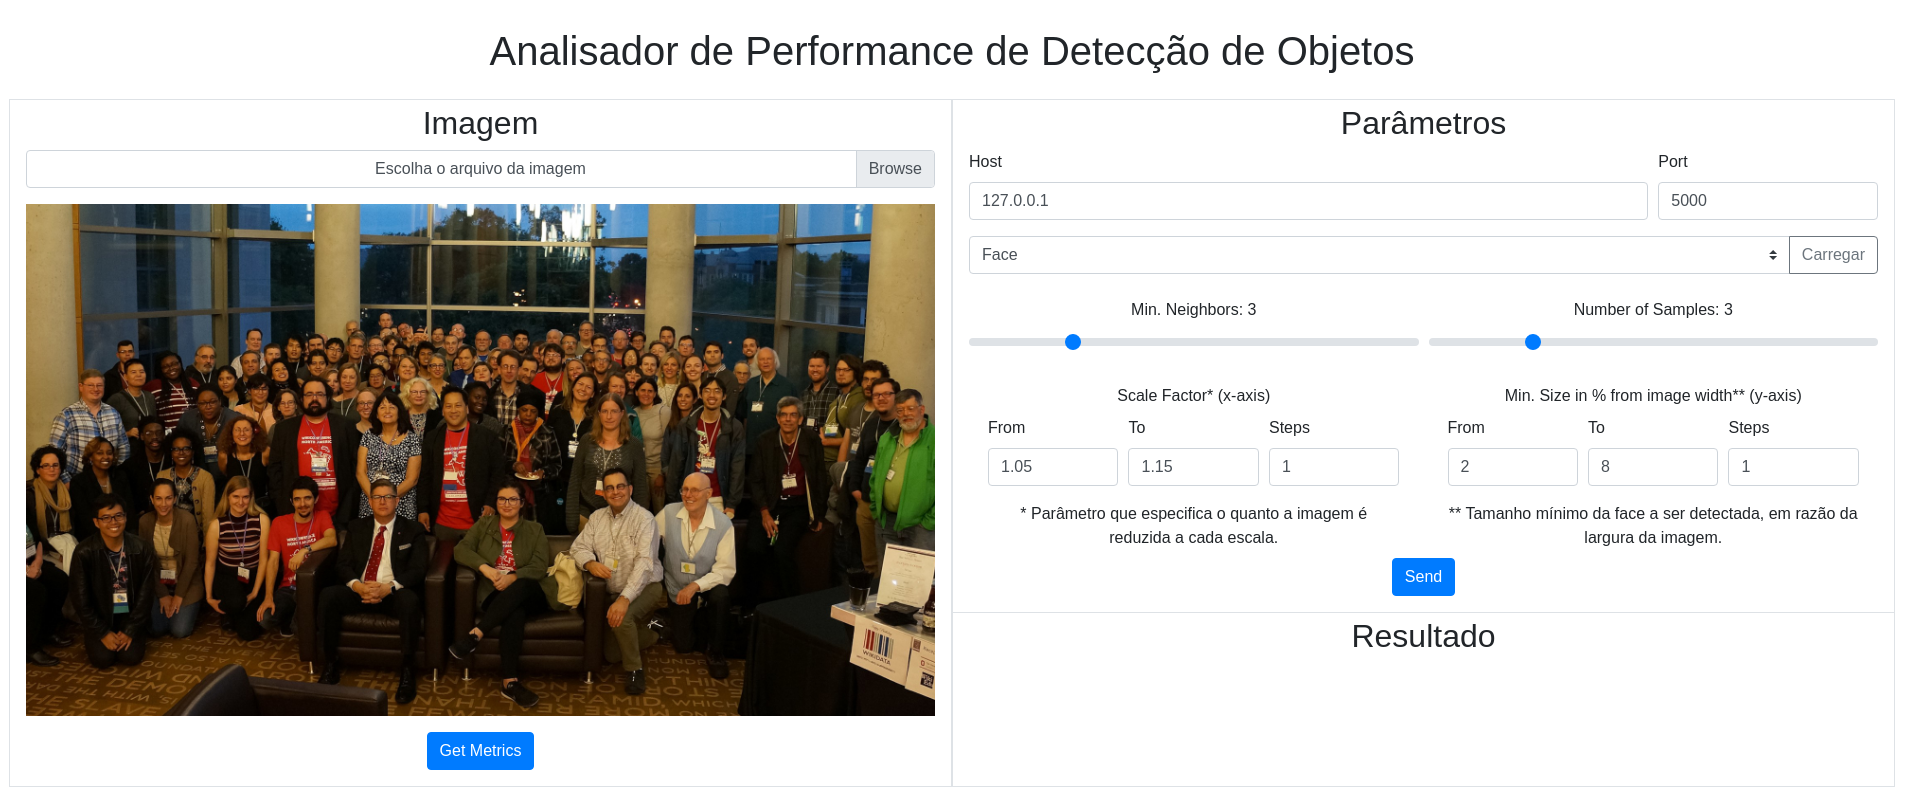
\includegraphics[width=1.0\textwidth]{Cap3_Desenvolvimento/Figures/interface_parametros.png}
    \caption*{Fonte: autor.}
    \label{fig:interfaceUsuario}
\end{figure}

<pending> fazer citação da imagem utilizada no exemplo></pending>

À esquerda da interface há um elemento de entrada que permite a seleção a imagem a ser utilizada no ensaio. Na imagem, exibida logo abaixo, serão delimitadas as faces detectadas.

À direita há dois campos, "Host" e "Port", que permitem a seleção do dispositivo a ser testado, a partir do endereço IP e porta em que a aplicação estará "escutando".

Logo abaixo estão os parâmetros a serem definidos e enviados ao servidor para a execução do ensaio. Três deles, "Scale factor", "Min neighbors" e "Min size", são parâmetros passados na própria função \textit{detectMultiScale} do OpenCV, e o significado de cada um foi descrito no início desta seção. O parâmetro "Number of Samples" determina quantas vezes o servidor executa cada combinação de parâmetros para obter um resultado médio.

Para o parâmetro "Min Neighbors", é possível definir apenas um valor para cada execução, que será utilizado em todas as combinações de parâmetros. Já para os parâmetros "Scale Factor" e "Min Size" é possível definir valores mínimos, máximos e as quantidade de valores ("Steps") a serem distribuidos linearmente nos intervalos definidos para cada um dos dois parâmetros. O servidor executará todas as combinações possíveis a partir dos conjuntos de valores delimitados, e retornará uma matriz com um resultado para cada combinação.

Por fim, ao se clicar no botão "Send", a imagem e os parâmetros são enviados para o servidor. O servidor executa o algoritmo de detecção com todas as combinações possíveis e retorna uma matriz de resultados contendo número de faces detectadas e tempo médio de execução.

\begin{figure}[h]
    \centering
    \caption[Exemplo de resultado retornado.]{Exemplo de resultado retornado.}
    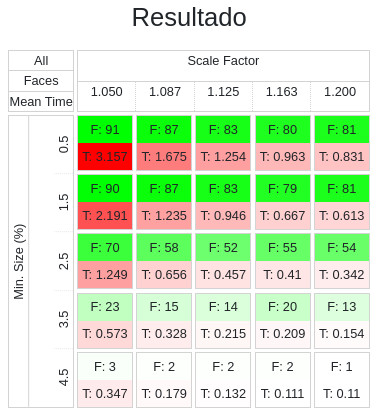
\includegraphics[width=0.6\textwidth]{Cap3_Desenvolvimento/Figures/exemplo_resultado_matriz.jpg}
    \caption*{Fonte: autor.}
    \label{fig:matrizResultado}
\end{figure}

Como pode ser visto na figura \ref{fig:matrizResultado}, o resultado é exibido em forma de uma matriz. No eixo vertical têm-se a distribuição dos valores definidos para o parâmetros "Min. Size" e no eixo horizontal têm-se a distribuição dos valores definidos para o parâmetro "Scale Factor", de conforme os limites e quantidades de passos definidos para cada um.

Cada célula da matriz apresenta o resultado da detecção, utilizando a combinação de parâmetros corresponde, com base em duas métricas, a quantidade de faces detectadas, na parte superior da célula, e o tempos médio em segundos, na parte inferior da célula. Importante ressaltar que o tempo médio refere-se ao tempo que o algoritmo levou para a detecção de todas as faces detectadas, e não ao tempo médio de execução de cada face. A média se dá de acordo com a quantidade de vezes que o algoritmo de detecção foi executado para cada combinação de parâmetros, definido em "Number of Samples".

Em uma primeira análise, a partir resultado do exemplo dado na figura \ref{fig:matrizResultado}, é possível observar a tendência de se ter maior quantidade de faces detectadas, bem como maior tempo de execução, quanto mais ao topo e à esquerda está a célula na matriz. Essa observação é um tanto óbvia tendo em vista que quanto menor o tamanho mínimo de faces a ser considerado pelo algoritmo (parâmetro "Min. Size"), mais faces candidatas tendem a ser encontradas e também mais iterações serão realizadas. O mesmo acontece para o parâmetro "Scale Factor", quanto menor o valor do parâmetro, menor o passo entre as escalas, maior a quantidade de imagens escalonadas avaliadas e, portanto, maior a chance de de uma determinada face ser detectada, bem como maior quantidade de iterações realizadas.

A matriz de resultados por si só não é suficiente para se determinar que uma combinação de parâmetros é a mais adequada a se adotar. Isso se deve ao fato de que não se pode afirmar que o resultado com o maior número de faces detectadas é o melhor pois, dentro do conjunto de faces detectadas, alguma poucas ou até várias delas podem ser falsos positivos, de tal forma que a qualidade do resultado da detecção deva ser considerado ruim. 

Outra questão a se considerar é que, dependendo do ambiente e do objetivo da aplicação, a detecção da maior quantidade de faces possível pode não ser a prioridade. Em determinado tipo de aplicação, pode ser mais interessante que o algoritmo detecte apenas faces que estejam mais próximas da câmera (e por conta disso relativamente maiores que as demais), com um tempo de resposta menor, do que detectar o máximo de faces possível, inclusive as mais distantes, que seriam descartadas, com um tempo de resposta maior.

Para tanto, é importante que haja uma análise qualitativa, ao se checar, para cada resultado analisado, quais foram as faces detectadas, resultantes da correspondente combinação de parâmetros. E, a partir da avaliação dos resultados disponíveis, comparando a presença de falsos positivos, a quantidade e tamanho das faces detectadas e o tempo médio de resposta, determinar uma combinação de parâmetros mais adequada a se adotar em uma aplicação de detecção no dispositivo testado ou concluir que o dispositivo não seria capaz de rodas a aplicação da forma desejada.

Para facilitar esse tipo de análise qualitativa, a matriz de resultados responde de forma interativa, de forma que, ao se clicar em uma célula da matriz, as faces detectadas a partir dos parâmetros correspondentes daquela célula são destacadas na imagem original através de retângulos verdes, facilitando assim a verificação de falsos positivos e quais faces presentes na imagem o algoritmo conseguiu detectar com tais parâmetros.

A seguir são apresentados alguns exemplos de resultados, a partir da matriz de resultado apresentada na figura \ref{fig:matrizResultado}. Para facilitar a visualização, serão apresentados apenas os cortes da matriz com o resultado selecionado e a imagem com as faces destacadas.

No exemplo da figura \ref{fig:exemploResultado1}, têm-se um resultado com muito poucas faces detectadas devido ao valor relativamente alto do parâmetro "Min. Size".

Já a figura \ref{fig:exemploResultado2} apresenta um resultado com várias faces detectadas, inclusive pequenas faces ao fundo. Porém, devido aos valores relativamente baixos dos parâmetros "Min. Size" e "Scale Factor", vê-se claramente a presença de três falsos positivos, além de um tempo médio de detecção consideravelmente alto, acima de 3 segundos.

Por fim, a figura \ref{fig:exemploResultado3} apresenta um resultado que possivelmente pode ser considerado satisfatório para determinados tipos de aplicação. Nesse caso, a maioria das faces presentes na imagem foi detectada e com um tempo de resposta razoavelmente baixo, pelo menos se comparado ao resultado apresentado na figura \ref{fig:exemploResultado2}.

\begin{figure}[h]
    \centering
    \caption[Exemplo de resultado com pucas faces detectadas.]{Exemplo de resultado com pucas faces detectadas.}
    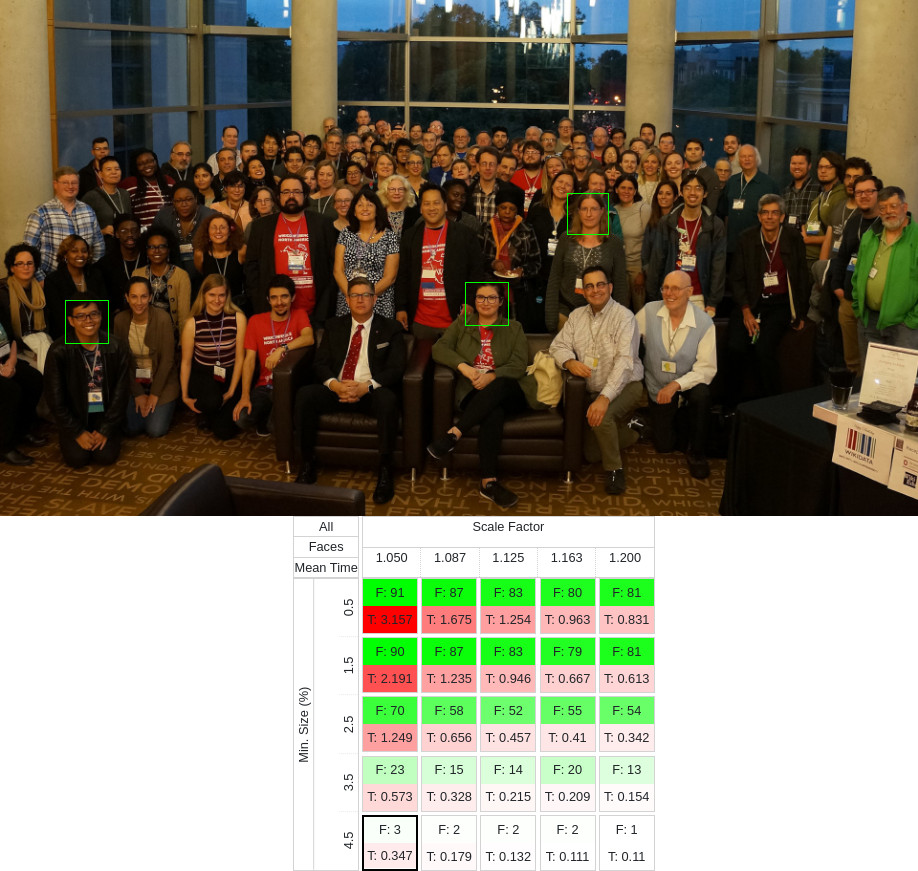
\includegraphics[width=0.8\textwidth]{Cap3_Desenvolvimento/Figures/exemplo_resultado_1.jpg}
    \caption*{Fonte: autor.}
    \label{fig:exemploResultado1}
\end{figure}

\begin{figure}[h]
    \centering
    \caption[Exemplo de resultado com várias faces detectadas e alguns falsos positivos.]{Exemplo de resultado com várias faces detectadas e alguns falsos positivos.}
    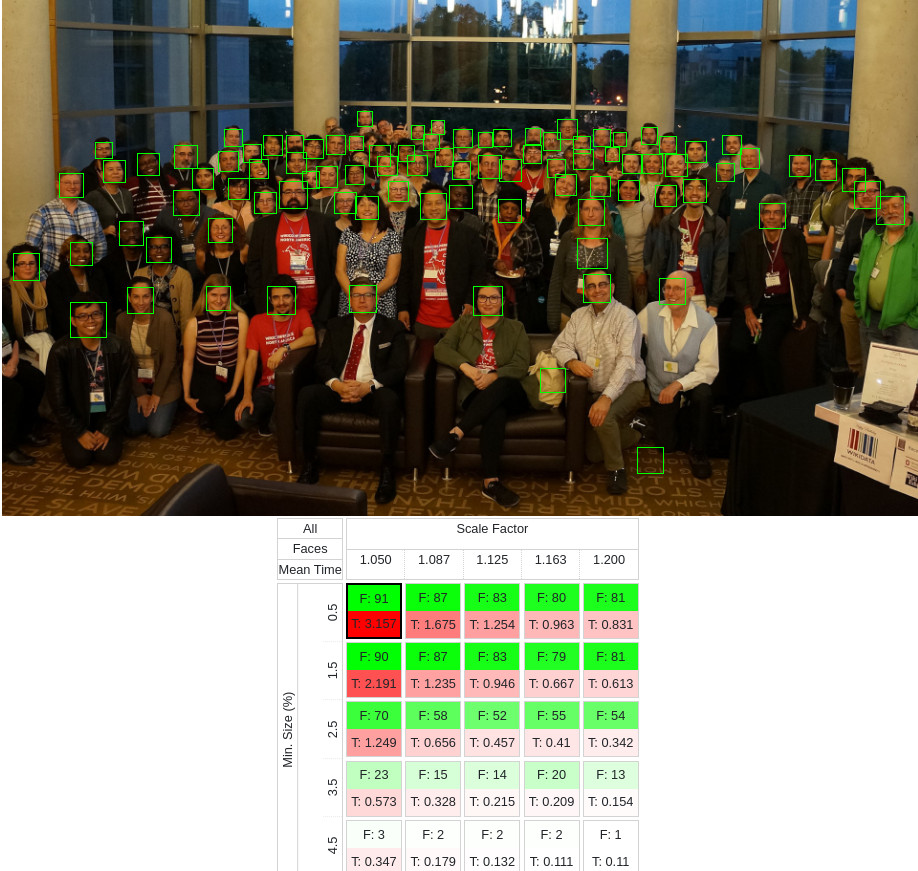
\includegraphics[width=0.8\textwidth]{Cap3_Desenvolvimento/Figures/exemplo_resultado_2.jpg}
    \caption*{Fonte: autor.}
    \label{fig:exemploResultado2}
\end{figure}

\begin{figure}[h]
    \centering
    \caption[Exemplo de resultado possivelmente satisfatório.]{Exemplo de resultado possivelmente satisfatório.}
    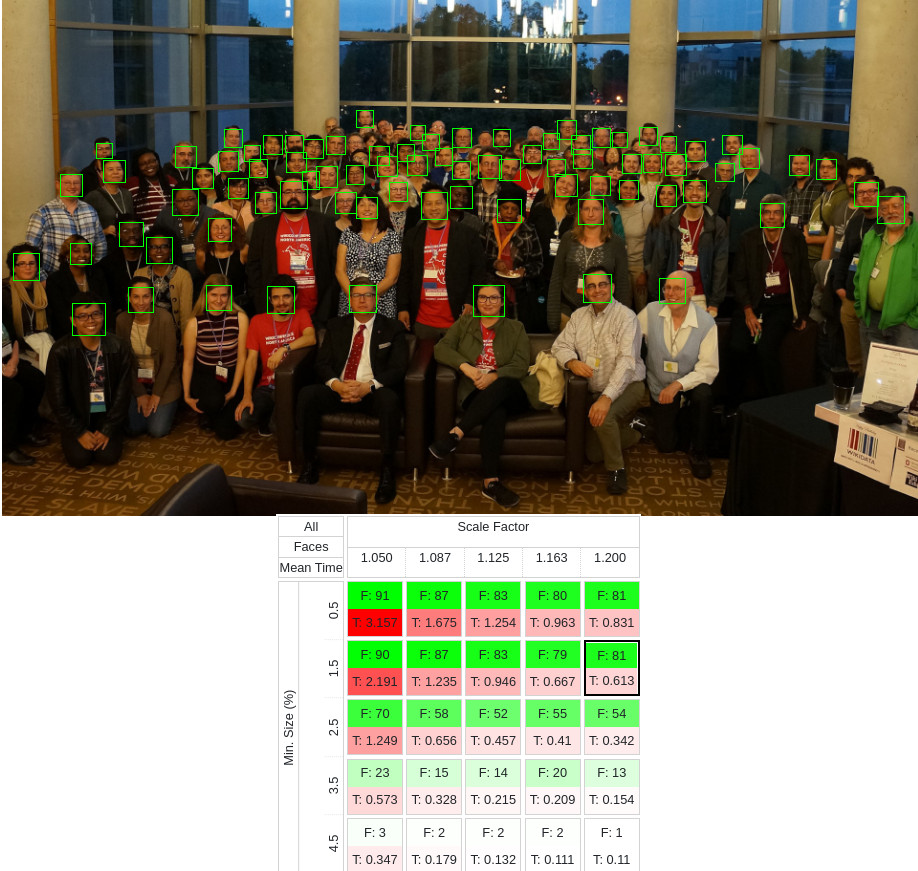
\includegraphics[width=0.8\textwidth]{Cap3_Desenvolvimento/Figures/exemplo_resultado_3.jpg}
    \caption*{Fonte: autor.}
    \label{fig:exemploResultado3}
\end{figure}


Outra facilidade que a ferramenta traz é quanto à flexibilidade na escolha dos limites e quantidades de valores a serem testados para cada parâmetros, permitindo, assim, ajustar os mesmos iterativamente, de forma a se ter cada vez melhores resultados e, consequentemente, melhores opções de otimização.

Ainda partindo da matriz de resultados da figura \ref{fig:matrizResultado}, alguns limites podem ser ajustados para uma próxima rodada de análise. Por exemplo, observa-se que nos resultados em que o valor de "Min. Size" é maior que 2.5, a quantidade de faces detectadas é muito baixa. Caso seja considerado insatisfatório, o novo valor máximo na distribuição desse parâmetro pode ser definido como 2.5 ou 3.0. Analisando o parâmetro "Scale Factor", pode-se observar que valores abaixo de 1.125 resultam em um tempo de resposta muito alto e apresenta muitos falsos positivos. Além disso, alguns resultados com o valor máximo apresentado de "Sacle Factor", 1.200, apresentam uma quantidade alta de faces detectadas, sendo possível que um valor maior possa apresentar um resultado igualmente bom mas com um tempo de resposta menor. Os limites de "Scale Factor" poderiam ser ajustados, por exemplo, para 1.080 e 1.250. Assim, uma próxima rodada de análise com os limites ajustados irão retornar uma maior e melhor gama de resultados.

A título de exemplo, a figura \ref{fig:matrizResultado2} apresenta a matriz de resultado com os limites ajustados. Observa-se uma melhor distribuição, com números de faces detectadas e tempo de resposta mais próximos do que podem ser considerados como satisfatórios, possibilitando uma análise mais precisa para determinar os melhores parâmetros.

\begin{figure}[h]
    \centering
    \caption[Exemplo de matriz de resultado com limites ajustados.]{Exemplo de matriz de resultado com limites ajustados.}
    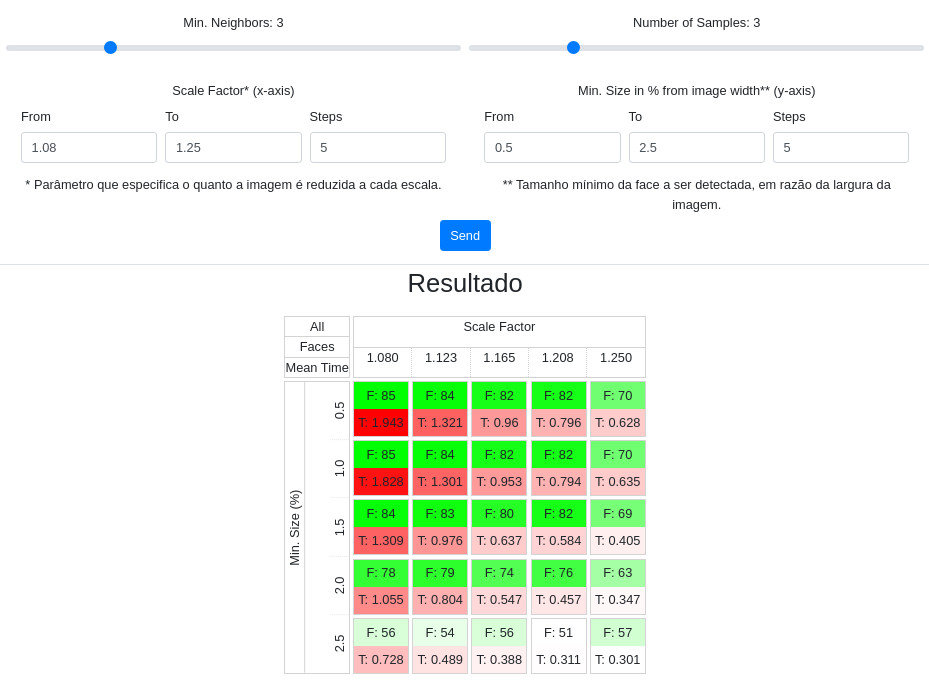
\includegraphics[width=0.8\textwidth]{Cap3_Desenvolvimento/Figures/exemplo_resultado_matriz_2.jpg}
    \caption*{Fonte: autor.}
    \label{fig:matrizResultado2}
\end{figure}

Há de se observar que, pelo fato de a análise estar sendo feita a partir de apenas uma imagem, não é de se esperar que o resultado quanto à presença, ou não, de falsos positivos, seja o mesmo para todos os frames que serão analisados em uma aplicaćão real, mesmo a câmera estando fixa, capturando sempre o mesmo cenário.

Em uma aplicação real da ferramenta, é interessante que os valores escolhidos dos parâmetros sejam testados utilizando-se outras imagens da mesma cena com suas possíveis variações, como por exemplo a diferente quantidade de pessoas e objetos, iluminações diferentes, etc.

Tendo definido-se uma melhor combinação de valores dos parâmetros, pode-se então obter uma análise mais aprofundada, com métricas adicionais, que auxiliará na análise e comparação dos resultados entre os diferentes cenários e dispositivos testados. Os resultados serão analisados considerando não só qualidade de deteção e tempo de reposta, como também a demanda de banda em rede e quantidade de dados trafegados para se progragar o resultado a uma próxima etapa de processamento dentro de um sistema distribuído.

Ao se clicar no botão "Get Metrics", no lado esquerdo da tela (vide figura \ref{fig:interfaceUsuario}), os parâmetros definidos de acordo com a célula selecionada na matriz de resultados são enviados ao servidor no dispositivo que está sendo testado. Este, por sua vez, executa novamente o algoritmo de detecção, logando também o tempo de execução de outras etapas preparatórias, bem como outras informações referentes aos tamanhos das imagens.

Na figura \ref{fig:resultadoMetricas}, pode-se observar como os dados retorandos são exibidos na interface do usuário. A seguir, uma breve explicação de cada item:

\begin{itemize}
    \item 1.0 - Params: os parâmetros utilizados no algoritmos de detecção, conforme célula selecionada na matriz de resultados na etapa anterior;
    \item 1.1 - Full Image Resolution: a resolução da imagem original, em pixels;
    \item 1.2 - Full Image Size (bytes): o tamanho da imagem original, em bytes;
    \item 1.3 - Full Image Encoded Size (bytes): o tamanho da imagem original codificada em bitmap e base64, em bytes;
    \item 1.4 - Number of detected faces: o número de faces detectadas;
    \item 1.5 - Cropped Faces Images Total Size (bytes) / (\% from full image size): o tamanho total das imagens de faces detectadas, recortadas da imagem original, em bytes, e o seu percentual com relaçãao ao tamanho da imagem original;
    \item 1.6 - Encoded Faces Images Total Size (bytes) / (\% from full image size): o tamanho total das imagens de faces detectadas, codificadas em bitmap e base64, em bytes, e o seu percentual com relação ao tamanho da imagem original codificada;
    \item 2.1 - Loading Image (s): o tempo de carregamento da imagem original (leitura em disco), em segundos;
    \item 2.2 - Convert Image to Gray (s): o tempo de conversão da imagem original para escala de cinza, em segundos. Etapa anterior necessária para execução do algoritmo de detecção;
    \item 2.3 - Detection (s): o tempo de execução do algoritmo de detecção em si, em segundos;
    \item 2.4 - Build Encoded Faces Images (s): o tempo de execução da etapa de encodamento das imagens em base64, em segundos;
    \item 2.5 - Total execution time (s): o tempo total de execução e todas as etapas, desde o carregamento da imagem até o encodamento em base64, em segundos.
    \item 3.1 - Faces images: as imagens das daces detectadas, recortadas da imagem original em seu tamanho real. Permite se ter uma ideia da qualidade de resolução individual das faces, bem como facilita a identificar mais facilmente a presença de falsos positivos que possam não terem sido identificados na etapa de análise anterior.
\end{itemize}

\begin{figure}[h]
    \centering
    \caption[Exemplo de resultado com as métricas.]{Exemplo de resultado com as métricas.}
    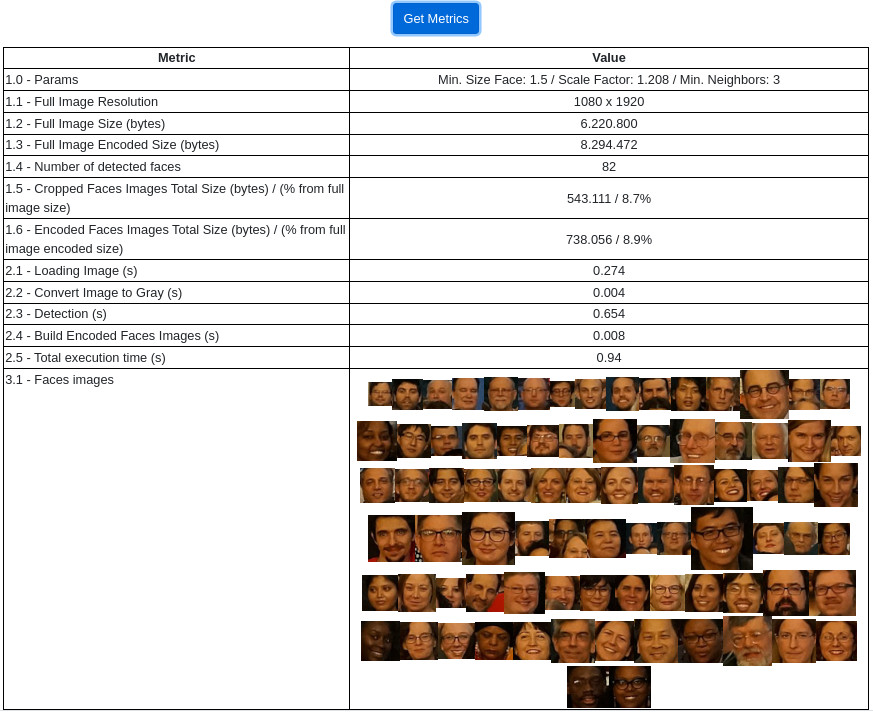
\includegraphics[width=0.8\textwidth]{Cap3_Desenvolvimento/Figures/exemplo_metricas.jpg}
    \caption*{Fonte: autor.}
    \label{fig:resultadoMetricas}
\end{figure}


\section{Cenários de testes}

Nesta seção são apresentados os cenários definidos para os testes. Cada cenário representa uma possível aplicação diferente e possui diferentes requisitos que servirão de balizas para a calibração e comparação dos resultados.

Para a realização do experimento, foram selecionadas imagens que representem um pior caso para cada cenário.

Para um estudo mais completo, serão testadas algumas variações de cada cenário, seja quanto à quantidade de faces presentes e/ou quanto à resolução da imagem testada, além, claro dos diferentes dispositivos que serão testados.

\subsection{Variação de quantidade de faces}

Em cenas cuja aplicação tenha como objetivo detectar um elevado número de faces simultaneamente, pretende-se verificar como a variação da quantidade de faces presente na imagem afeta tanto no tempo de resposta do processo de detecção quanto no tamanho do conjunto das imagens das faces detectadas, recortadas da imagem completa, representando economia na utilização de banda para transmissão do resultado da detecção.

Para a realização desses testes nas cenas a que a variação da quantidade de faces se aplica, foram selecionadas imagens com um grande número de faces, para que se possa obter tranquilamente 5 variações da mesma imagem, reduzindo iterativamente a quantidade de faces em cada uma, da forma mais linear possível.

As variações foram preparadas utilizando-se o software de edição de imagem GIMP (GNU Image Manipulation Program), aberto e gratuito. Partindo-se da imagem original, uma certa quantidade de faces foram borradas de forma a se tornarem indetectáveis, como se aquela faces não estivessem presentes na imagem. A imagem resultante se tornou a primeira variação por quantidade de faces. A partir da imagem dessa primeira variação, foi feito o mesmo procedimento, borrando a mesma quantidade de faces que ainda não haviam sido borradas. E assim foi feito sucessivamente até obter-se um total de 5 variações. Importante ressaltar que, durante a preparação das imagens, preocupou-se em borrar as faces de uma forma bem distribuída.

\begin{figure}[h]
    \centering
    \caption[Exemplo de variação de cena com redução de 20 faces.]{Exemplo de variação de cena com redução de 20 faces.}
    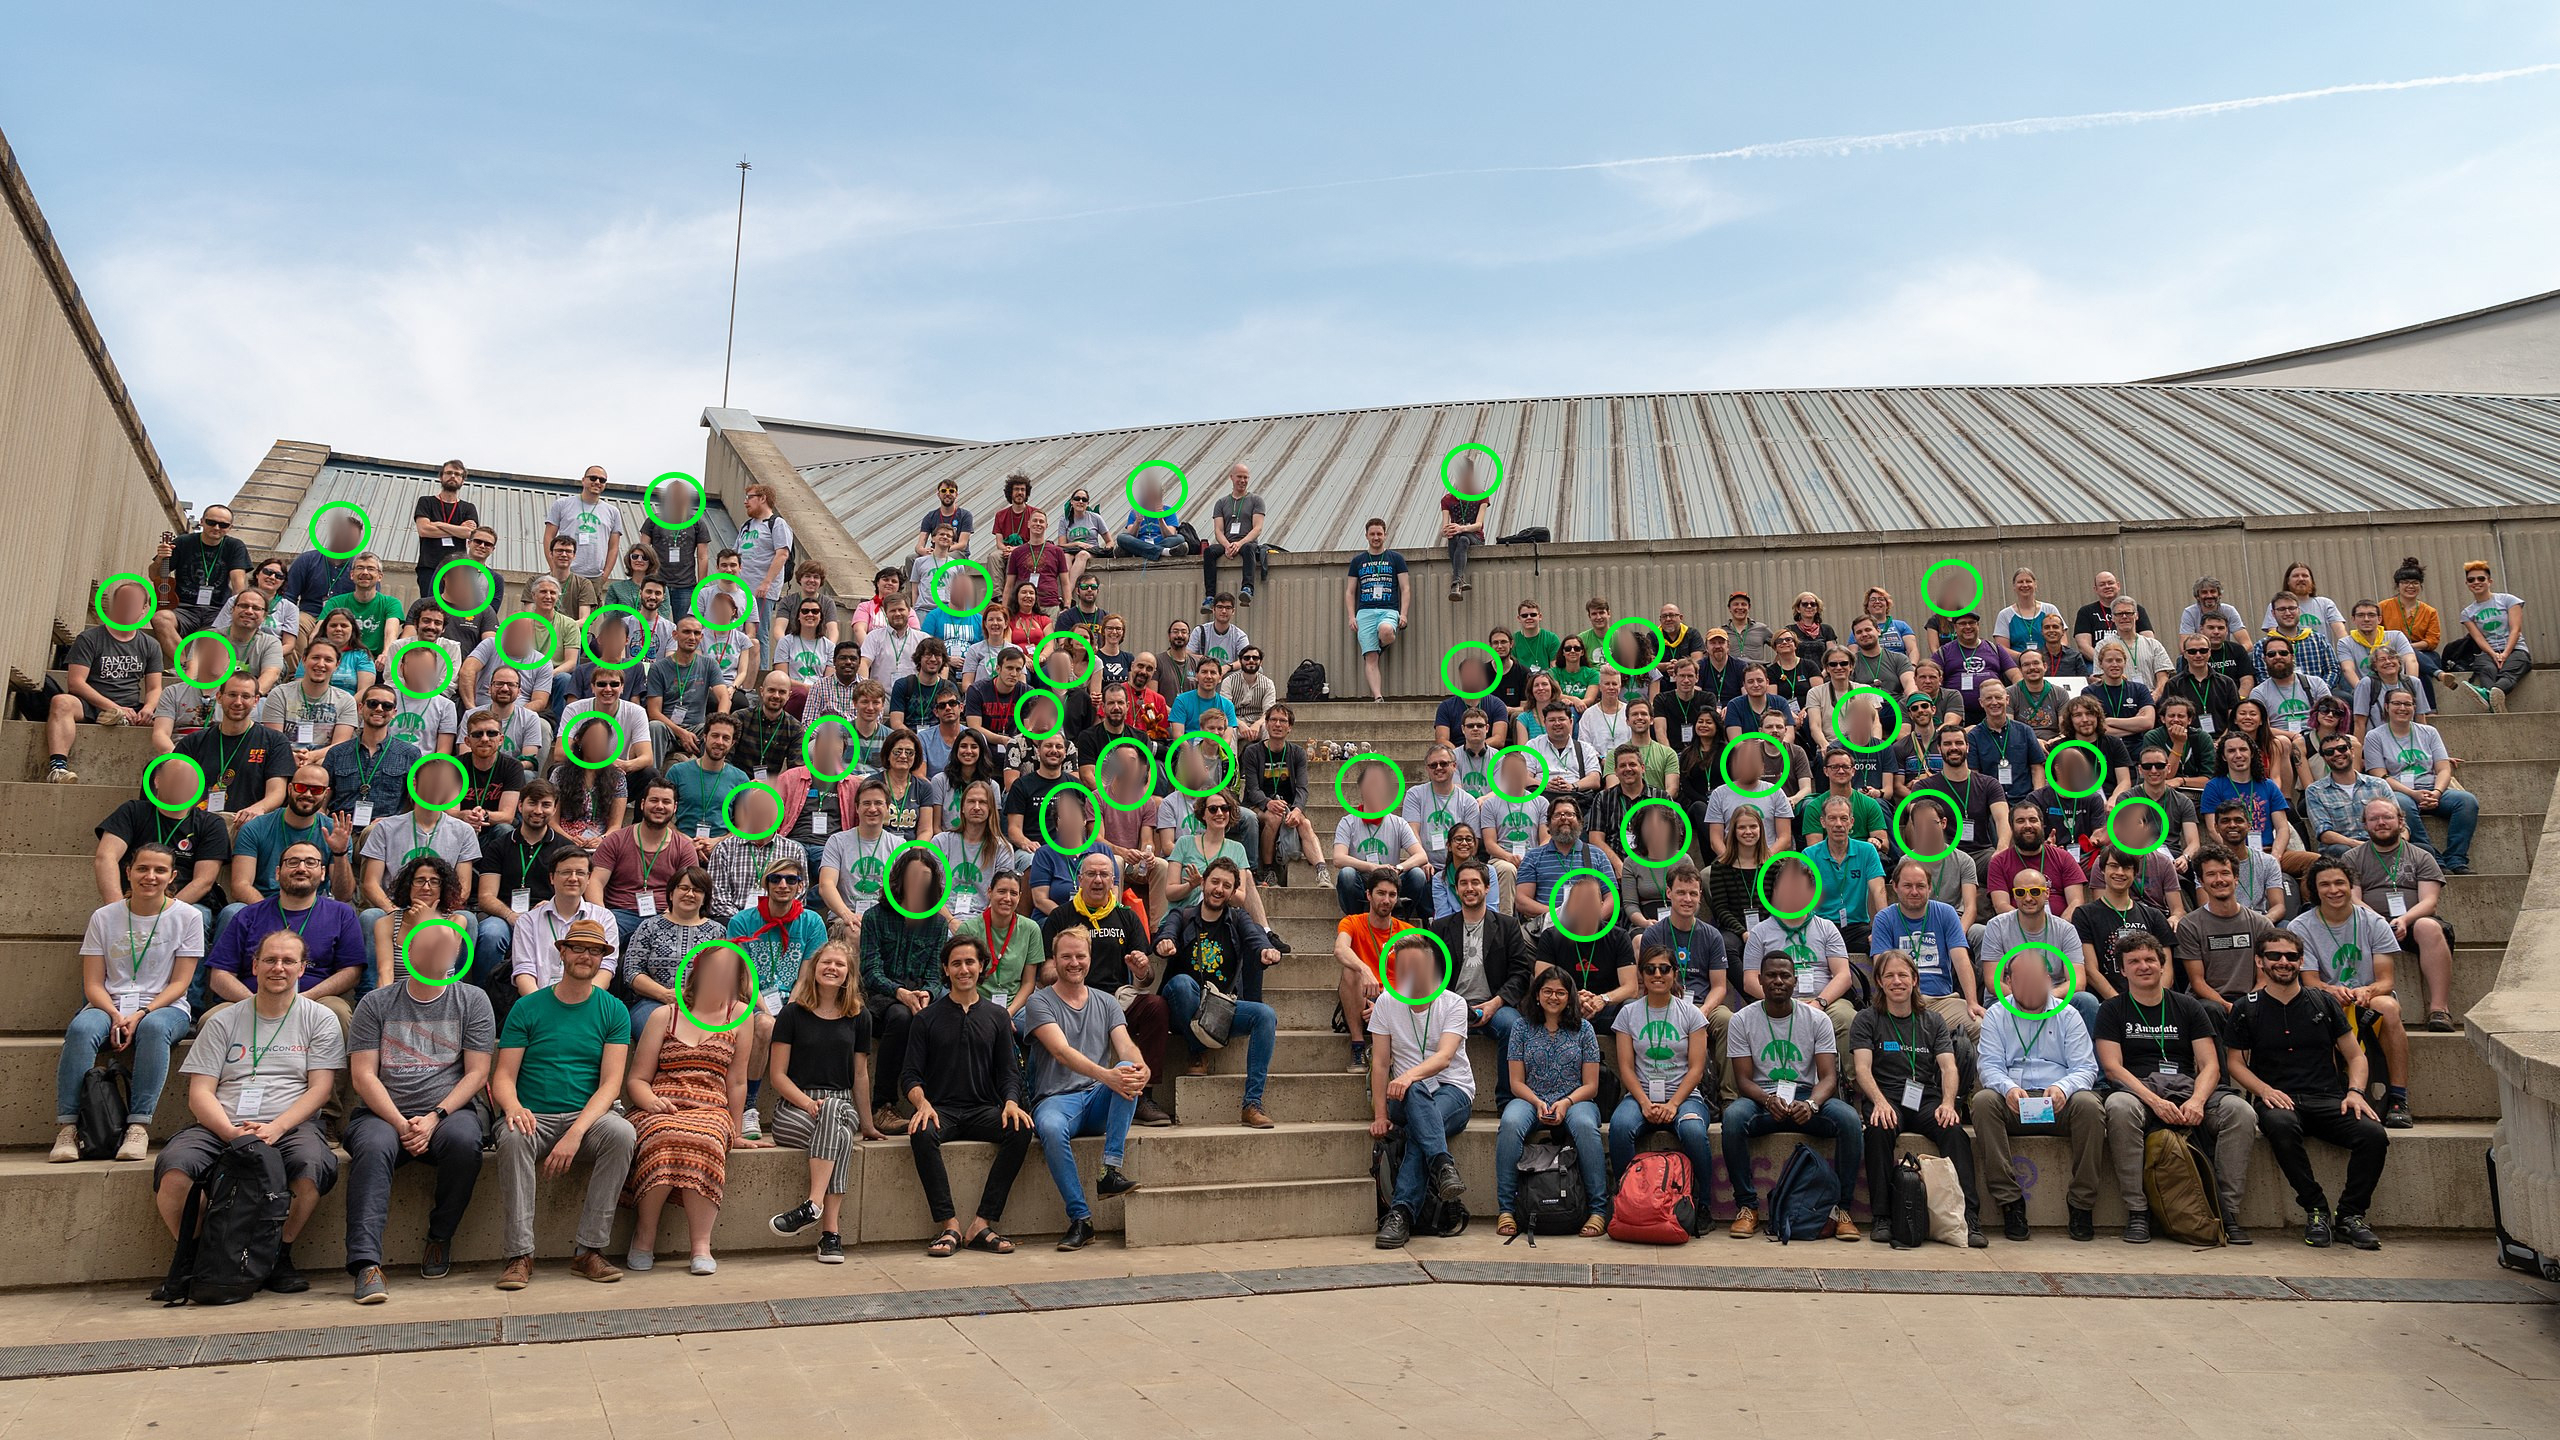
\includegraphics[width=0.8\textwidth]{Cap3_Desenvolvimento/Figures/exemplo_variacao_faces.png}
    \caption*{Fonte: autor.}
    \label{fig:exemploVariacaoFaces}
\end{figure}

Na figura \ref{fig:exemploVariacaoFaces}, um exemplo de variação com a redução de 20 faces. Ao se comparar o resultado das variações, é de se esperar que a diferença de faces detectadas seja igual à diferente da quantidade de faces borradas, porém, não necessariamente será igual, pois pode ser que alguma face não seja detectada pelo algoritmo de qualquer forma.

Para obtenção dos dados nos testes de variação de quantidade de faces deve-se, a partir da imagem original, com todas as faces detectáveis, utilizar a ferramenta para encontrar uma combinação otimizada de parâmetros de detecção. Com os melhores parâmetros definidos, obtém-se as métricas da imagem original e também de todas a variações de quantidade de faces geradas a partir dessa mesma imagem para futura comparação.

\subsection{Variação de resolução da imagem}

Outra variação que é possível obter de uma mesma imagem e que fará parte do estudo é no que tange à resolućão da imagem. Quanto maior a resolução da imagem, maior tende a ser a capacidade e qualidade de detecção de faces menores, mas também maior é a demanda de processamento e maior tende a ser o tempo de espera de uma detecção, bem como a utilização de banda para passar adiante as imagens das faces detectadas.

Dependendo do cenário e dos possíveis tipos de aplicação, considerar trabalhar a decção em imagens com resoluções menores que a capacidde do sensor, pode ser suficiente para viabilizar o uso do dispositivo de borda para a tarefa de detecção, desde que cumprindo os requisitos de tempo de resposta e capacidade de detecção.

Para a realização dos testes com variação de resolução, foram obtidas das imagens originais (a original e suas respectivas variações por quantidade de faces) imagens com resoluçoes menores, através de interpolação, utilizando-se também o software GIMP para o processamento. As imagens originais de cada cena foram selecionadas já com resolução em full hd (1920x1080), e foram obtidas as variações nas resoluçoes hd (1280x720) e sd (720x480). Para cada redução de resolução, são obtidas 5 novas imagens, uma a partir da imagem original e outras quatro a partir da variações de quantidade de faces.

Para a obtenção dos dados nos testes de variação de resolução, deve-se utilizar novamente a ferramenta para encontrar a melhor combinação de parâmetros de detecção para as imagens na nova resolução e, a partir desses novos parâmetros, obter as métricas de todas as imagens com a referida resolução.

\subsection{Dispositivos testados}

Serão testados três dispositivos SBC \textit{Single Board Computer} diferentes, cujos resultados serão comparados.

\begin{itemize}
    \item SBC 1 - Raspberry Pi 4: quad-core Cortex-A72 com clock de 1,5 GHz e 4 GB de memória RAM LPDDR4. 
    \item SBC 2 - Raspberry Pi Zero: ...
    \item SBC 3 - ...
\end{itemize}

\subsection{Cena 1}

Nessa primeira cena deseja-se representar o monitoramento de um espaço aberto e amplo, onde é esperado um fluxo alto de pessoas e que estas possam estar a qualquer distância da câmera, sendo desejável que o dispositivo consiga detectar faces muito pequenas a ponto de maximar quantidade de faces detectadas.

\begin{itemize}
    \item \textbf{Variações possíveis} - variação de quantidade de faces e variação de resolução da imagem.
    \item \textbf{Requisitos mínimos} (para balizar a parametrização) - máximo 3 segundo de resposta.
    \item \textbf{Imagem para testes} - para representar esta cena, foi selecionada uma imagem (figura \ref{fig:imagemCena1}) com várias faces olhando na direção da câmera e em diferentes distâncias. Ter todas as faces olhando para a mesma direção distancia de um cenário real, mas se torna ideal para o estudo pois serve como um pior caso para a cena e facilita a obtenção de variações por quantidade de faces.
\end{itemize}

\begin{figure}[H]
    \centering
    \caption[Imagem selecionada para testes da cena 1.]{Imagem selecionada para testes da cena 1.}
    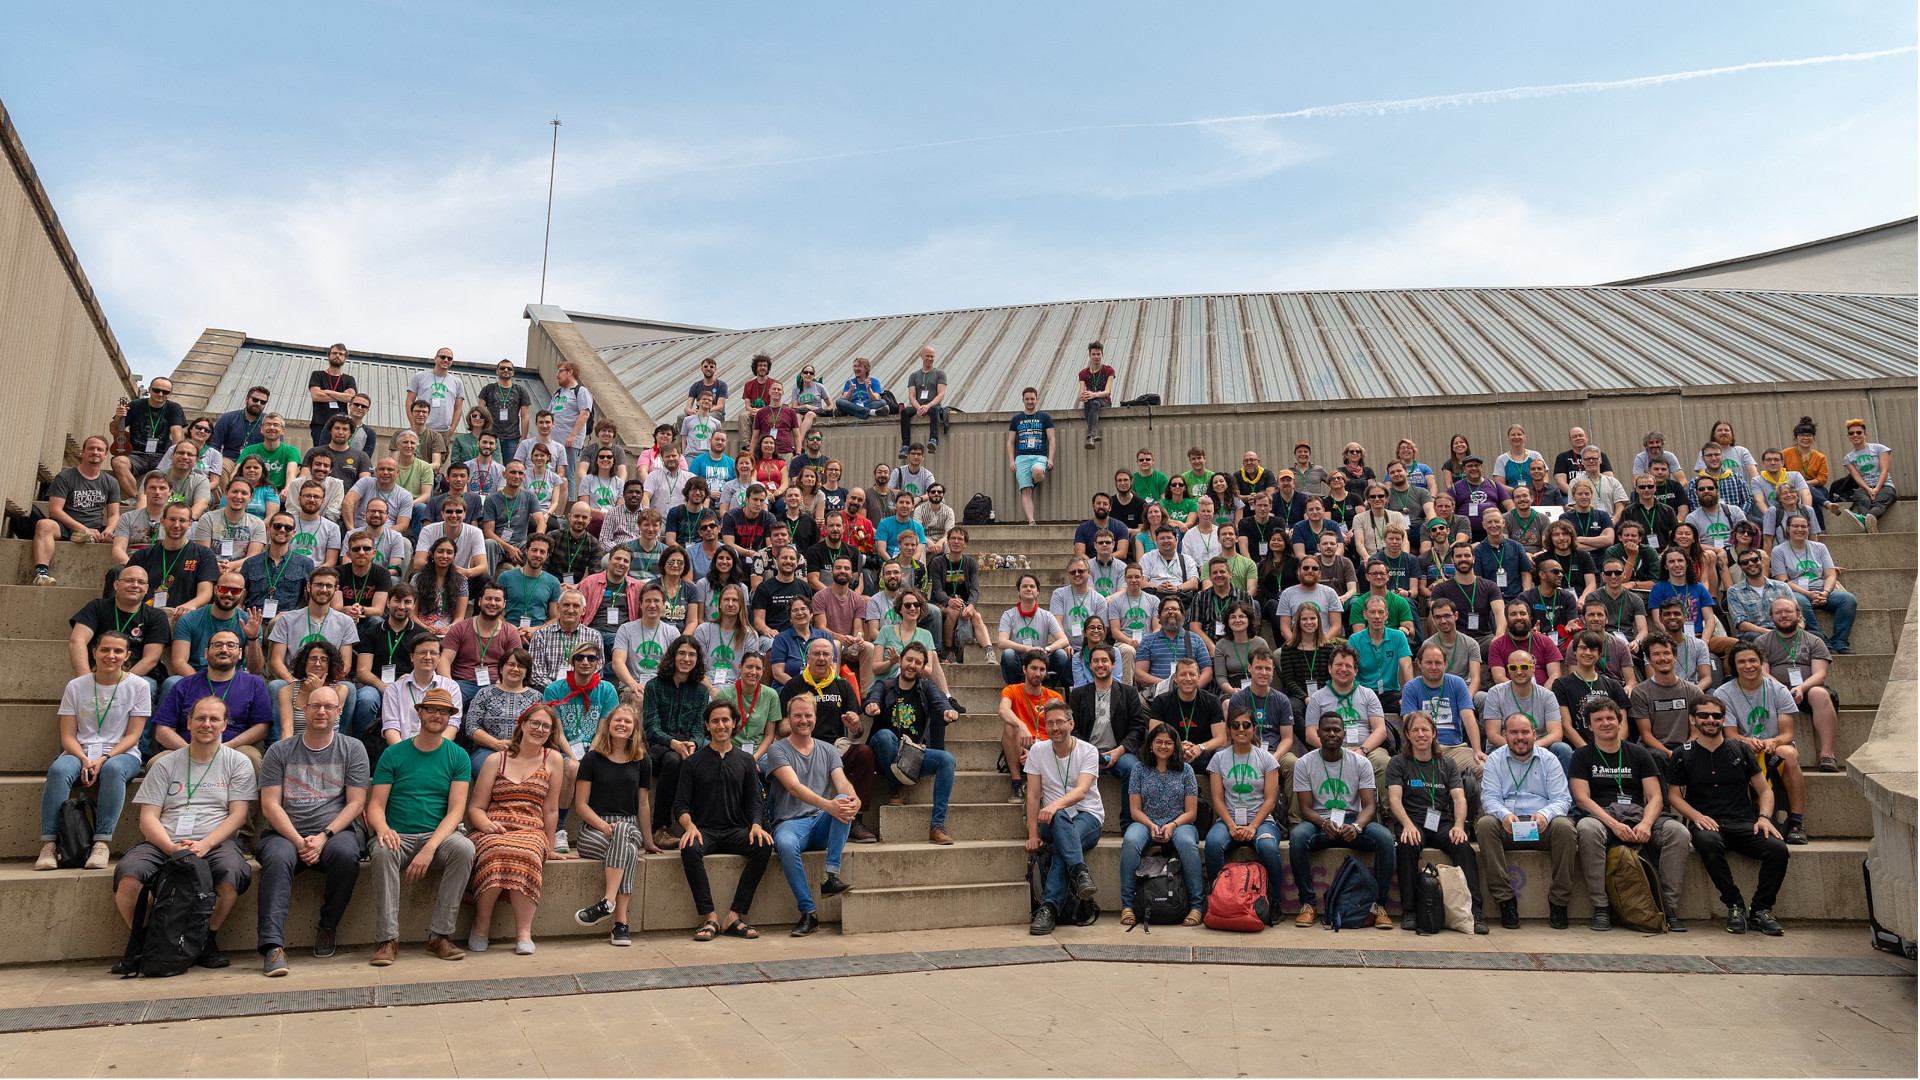
\includegraphics[width=0.8\textwidth]{Cap3_Desenvolvimento/Figures/imagem_cena1.jpg}
    \caption*{Fonte: Wikimedia Hackathon Barcelona 2018, por Ckoerner, 2018\footnotemark.}
    \label{fig:imagemCena1}
\end{figure}

\footnotetext{Disponível em: <https://commons.wikimedia.org/wiki/File:Wikimedia\_Hackathon\_Barcelona\_2018\_-\_group\_photo.jpg>

Arquivo de imagem sob a licença CC BY-SA 4.0: <https://creativecommons.org/licenses/by-sa/4.0/deed.en>}
\chapter{Experimentos Realizados}
\thispagestyle{plain}
\label{cap:experimentos}
\graphicspath{{./Cap4_Experimentos_Realizados/Figures/}}

A realização dos experimentos baseou-se na utilização da ferramenta de parametrização e obtenção de métricas, aplicado nas imagens tratadas de cada cena, conforme variaçoes definidas no Capítulo anterior. Os dados obtidos foram organizados de forma a facilitar a análise e comparação entre as variaçoes em cada cena e também entre os diferentes dispositivos sendo testados.

Para cada variação de resolução, que depende de uma nova seleção de parâmetros, será exibido a matriz de resultados final juntamente com as faces detectadas, após já feita a análise para se chegar a um melhor resultado, indicando quais foram os parâmetros definidos.

\section{Cena 1}

\subsection{Otimização de parâmetros}

Primeiramente, foi realizada a otimização dos parâmetros para cada variação de resolução, a partir das imagens com todoas as faces disponíveis de cada resolução.

A definição dos parâmetros 'ótimos' não é objetiva. Para esta cena, buscou-se um melhor resultado em que houvesse a maior quantidade de faces detectadas sem a presença de falsos positivos e no menor tempo. Durante a análise, teve-se a razoabilidade de considerar na comparação entre os diferentes resultados da matriz que, um grande aumento no tempo de detecção não justifica um pequeno ganho relativo na quantidade de faces detectadas.

\subsubsection{Resolução 1440p}

\begin{figure}[h]
    \centering
    \caption[Otimização Cena1 resolução 1440p.]{Otimização Cena1 resolução 1440p.}
    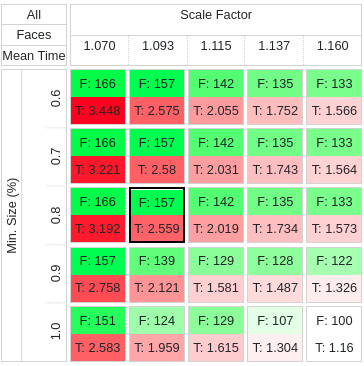
\includegraphics[width=0.4\textwidth]{Cap4_Experimentos_Realizados/Figures/cena1_param_1440p_matriz.jpg}
    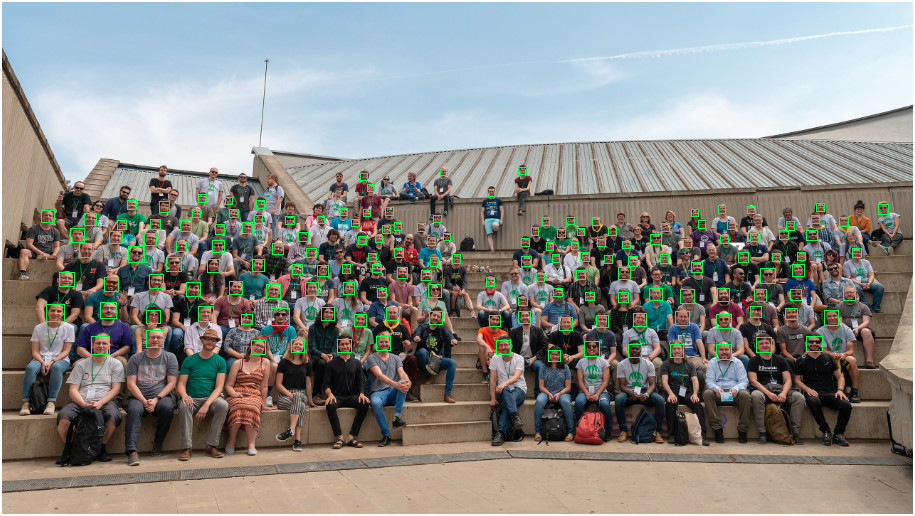
\includegraphics[width=1.0\textwidth]{Cap4_Experimentos_Realizados/Figures/cena1_param_1440p_faces.jpg}
    \caption*{Fonte: autor.}
    \label{fig:otimizacaoCena1_1440p}
\end{figure}

\subsubsection{Resolução 1080p}

\begin{figure}[h]
    \centering
    \caption[Otimização Cena1 resolução 1080p.]{Otimização Cena1 resolução 1080p.}
    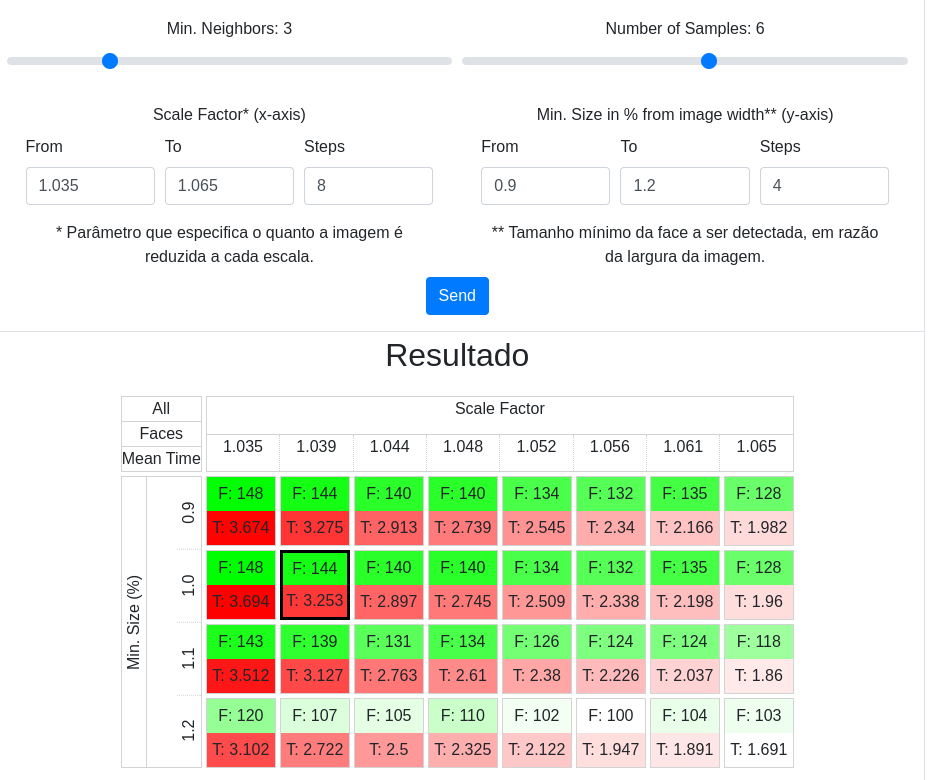
\includegraphics[width=0.4\textwidth]{Cap4_Experimentos_Realizados/Figures/cena1_param_1080p_matriz.jpg}
    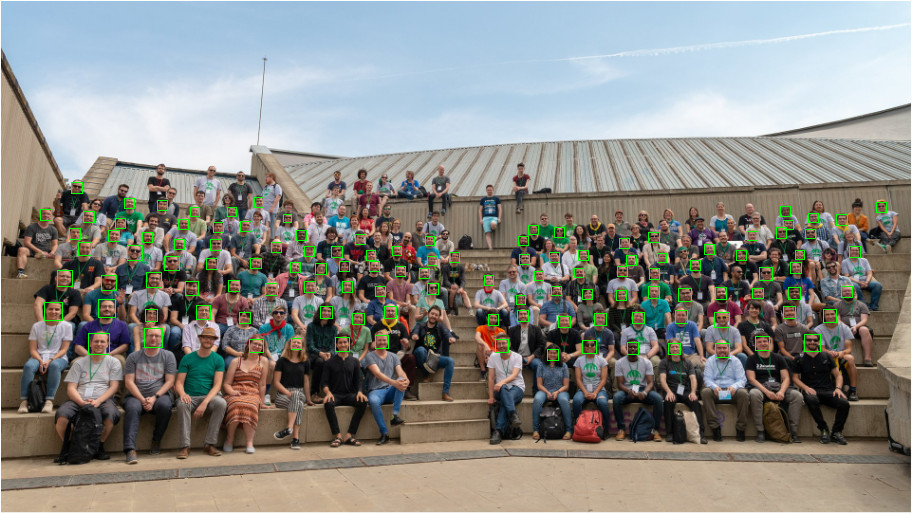
\includegraphics[width=1.0\textwidth]{Cap4_Experimentos_Realizados/Figures/cena1_param_1080p_faces.jpg}
    \caption*{Fonte: autor.}
    \label{fig:otimizacaoCena1_1080p}
\end{figure}

\subsubsection{Resolução 720p}

\begin{figure}[h]
    \centering
    \caption[Otimização Cena1 resolução 720p.]{Otimização Cena1 resolução 720p.}
    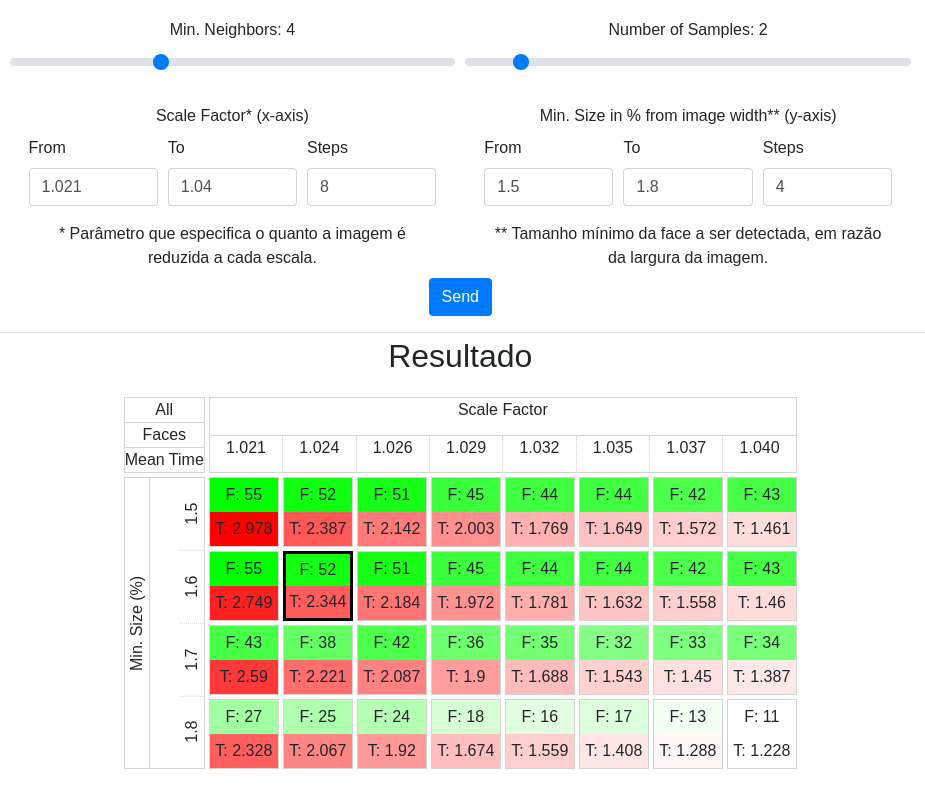
\includegraphics[width=0.4\textwidth]{Cap4_Experimentos_Realizados/Figures/cena1_param_720p_matriz.jpg}
    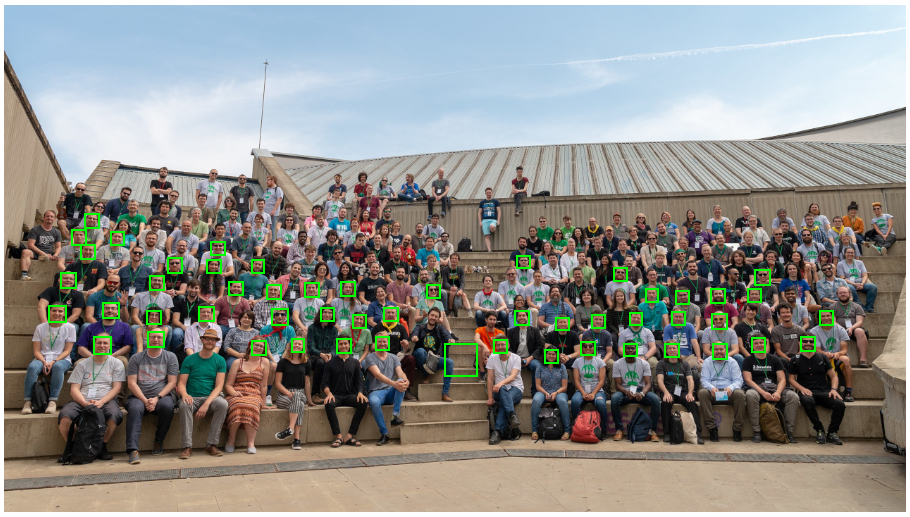
\includegraphics[width=1.0\textwidth]{Cap4_Experimentos_Realizados/Figures/cena1_param_720p_faces.jpg}
    \caption*{Fonte: autor.}
    \label{fig:otimizacaoCena1_720p}
\end{figure}
\chapter{Considerações Finais e Trabalhos \mbox{Futuros}}\label{cap:conclusao}
\thispagestyle{plain}



\bibliography{minhasReferencias}



\end{document}
